% 美赛模板:正文部分
\documentclass[12pt]{article}  % 官方要求字号不小于 12 号,此处选择 12 号字体
\linespread{1.2}
% \bibliographystyle{plain}
% 本模板不需要填写年份,以当前电脑时间自动生成
% 请在以下的方括号中填写队伍控制号
\usepackage[2501909]{easymcm}  % 载入 EasyMCM 模板文件
\problem{A}  % 请在此处填写题号
\usepackage{mathptmx}  % 这是 Times 字体,中规中矩 
% \usepackage{palatino}  % mathpazo 这palatino是 COMAP 官方杂志采用的更好看的 Palatino 字体,可替代以上的 mathptmx 宏包
\usepackage{pdfpages}
\usepackage{longtable}
\usepackage{tabu}
\usepackage{threeparttable}
\usepackage{listings}
\usepackage{paralist}
\usepackage{setspace}
\usepackage{array}
\usepackage{amsmath} 
\usepackage{hyperref}
\usepackage{subcaption}
%\renewcommand{\subfigureautorefname}{Figure} %子图片引用前缀,忽略报错!!!
\numberwithin{equation}{section} %公式按照章节编号

 \let\itemize\compactitem
 \let\enditemize\endcompactitem
% \let\enumerate\compactenum
% \let\endenumerate\endcompactenum
% \let\description\compactdesc
% \let\enddescription\endcompactdesc
% \usepackage{biblatex} 
% \usepackage{cite}
% \usepackage{natbib}
\newcommand{\upcite}[1]{\textsuperscript{\textsuperscript{\cite{#1}}}}
\title{XXXXXX}  % 标题

% 如需要修改题头(默认为 MCM/ICM),请使用以下命令(此处修改为 MCM)
%\renewcommand{\contest}{MCM}

% 文档开始
\begin{document}
\begin{abstract}
	
	% (Need to be reviewed)
	XXX
	
	XXX
        
    For task1: XXX	

    For task2: XXX

    For task3: XXX

   
	% Firstly, that is ...
	% Secondly, that is ...
	% Finally, that is ...	
	% 美赛论文中无需注明关键字。若您一定要使用,
	% 请将以下两行的注释号 '%' 去除,以使其生效
	\vspace{5pt}
	\textbf{Keywords}: XXX, XXX, XXX, XXX
	
\end{abstract}
\maketitle  % 生成 Summary Sheet
\tableofcontents


% 正文开始
% Chapter 1: Introduction
\section{Introduction}

\subsection{Problem Background}
As a symbol of permanence, stone is often used for building components. Despite its durability, the stone is not impervious. As people walk up and down over time, steps are molded into different shapes that tell stories of the past, waiting to be explored.

The wear on stairs reflects the behavioral patterns of people in the past. Long-term behavior of people is likely to have subjected the steps to uneven wear, leaving the treads with curved tops. For example, in ancient temple staircases, the centers of the steps are more worn than the edges. Archaeologists are interested in the age, the traffic patterns, and the frequency of use of stairs. But the presence of people and the temporal variability in the construction of the staircase, and the renovation of the staircase have obscured some of this information.
\begin{figure}[H]
	\centering
	\includegraphics[width=0.75\linewidth]{美赛Latex模板/image1.png}
	\caption{Worn stone steps}
	\label{stair1}
     \vspace{-2em} % 用来调间距
\end{figure}

To assist the archaeologists, the team was asked to build relevant mathematical models for the following tasks:

\textbf{Task1:} Given a set of stairs, develop a mathematical model that considers the wear patterns of a particular staircase. Provide some basic predictions:
\begin{itemize}
	\setlength{\parsep}{0ex} %段落间距
	\setlength{\topsep}{0ex} %列表到上下文的垂直距离
	\setlength{\itemsep}{0ex} %条目间距
	\item Discuss the frequency of use of this staircase.
	\item Explore the direction of travel favored by the people using the stairs.
	\item Study how many people use the stairs at the same time.
\end{itemize}

When archaeologists are skeptical about a staircase, field measurements can be made. A non-destructive surveying program, which requires minimum cost, fewer people, and the fewest tools can be taken.

\textbf{Task2}: Further problem solving. By using the available estimates, determine what guidance can be provided for the following questions:
\begin{itemize}
	\setlength{\parsep}{0ex} %段落间距
	\setlength{\topsep}{0ex} %列表到上下文的垂直距离
	\setlength{\itemsep}{0ex} %条目间距
	\item The consistency of wear with available information.
	\item The age of the stairwell and the reliability of the estimate.
	\item The repairs or renovations have been made to the stairwell.
    \item Determine the provenance of materials and compare them with the speculations of archaeologists.
    \item Analyses the use of the stairwell on a typical day.
\end{itemize}

\subsection{Our work}
To summarize the article, we have:
\begin{enumerate}[\bfseries (1)]
	\setlength{\parsep}{0ex} %段落间距
	\setlength{\topsep}{2ex} %列表到上下文的垂直距离
	\setlength{\itemsep}{1ex} %条目间距
	\item 
	\item 
	\item 
	\item 
\end{enumerate}

% Chapter2 : 模型假设
\section{Assumptions and Notations}
%\vspace{-1.5em}
\subsection{Assumptions}
%\vspace{-1.0em}
To simplify the problem and make it convenient for us to simulate real-life conditions,we make the following basic assumptions, each of which is properly justified.
\begin{itemize}
	\setlength{\parsep}{0ex} %段落间距
	\setlength{\topsep}{2ex} %列表到上下文的垂直距离
	\setlength{\itemsep}{1ex} %条目间距
	\item \textbf{Assumption 1:}XXX\\
    \textbf{Justification:}XXX.
    \item \textbf{Assumption 2:}XXX \\
    \textbf{Justification:}XXX 
    \item \textbf{Assumption 3:} XXX\\
    \textbf{Justification:} XXX
    \item \textbf{Assumption 4:} XXX\\
    \textbf{Justification:} XXX

\end{itemize}

% Chapter3 : 符号说明
\vspace{-1.0em}
\subsection{Notations}
\begin{table}[H]
\vspace{-2.0em}
	\centering
        \caption{Notations Table}
        \renewcommand{\arraystretch}{1.5}
        \setlength{\tabcolsep}{16pt}
	\begin{tabular}{cc}
		\hline
		\hline
		\multicolumn{1}{c}{\textbf{Notations}} & \textbf{Definition}\\ \hline
        $d(x,y)$                       & The wear depth at point (x, y) on the stone step\\
		$T$                      & The construction duration of the stair
\\
		$N_d$                      & The average number of people walking on the staircase per day\\
		$G$                       & The average gravitational force experienced by walking people\\
        $k_m$                       & The amount of wear caused by unit force on the stone step\\
        $D(x,y)$                       & The foot traffic rate contributing to wear at point (x, y) on the stone step\\
        $k_m$                       & The wear coefficient of the material\\
        $d$                       & The sliding distance of contact on the tread surface of the step\\
        $H$                       & Material hardness\\
        
    \hline
		\hline
	\end{tabular}
\end{table}


\section{Stair Wear Model}
According to assumptions 1 and 2, people all use the single-step strategy (SS) to walk on the stairs. The rest of the factors have the same effect on the given set of steps. Therefore, in the absence of repairs, the condition of a single stone step gives a good picture of the age of a given set of steps, the traffic patterns of the people, and the daily patterns of life.  To acquire this interest information to archaeologists, we model the  Wear Volume Model and the Wear Distribution Model. Besides, we present the data that need to be measured. Finally, a set of ancient sandstone steps in Edinburgh is used as an example for solving the problem.
\subsection{Wear Volume Model}
\subsubsection{Rasterize the surface of the step}
In order to represent the actual physical steps using a mathematical model for easy computer processing, we rasterize the steps. As shown in \label{Rasterization}, we take the top view of a step to obtain a rectangle with length $X$ m and width $Y$ m, which is discretized and divided into $m\times{n}$ rasters.

%\begin{figure}[H]
%	\centering
%	\includegraphics[width=0.9\linewidth]{美赛Latex模板/img/Rasterization.png}
%	\caption{Rasterized diagram of the stair surface}
%	\label{Rasterization}
%    \vspace{-2em} % 用来调间距
%\end{figure}

\begin{figure}[H]
	\centering
	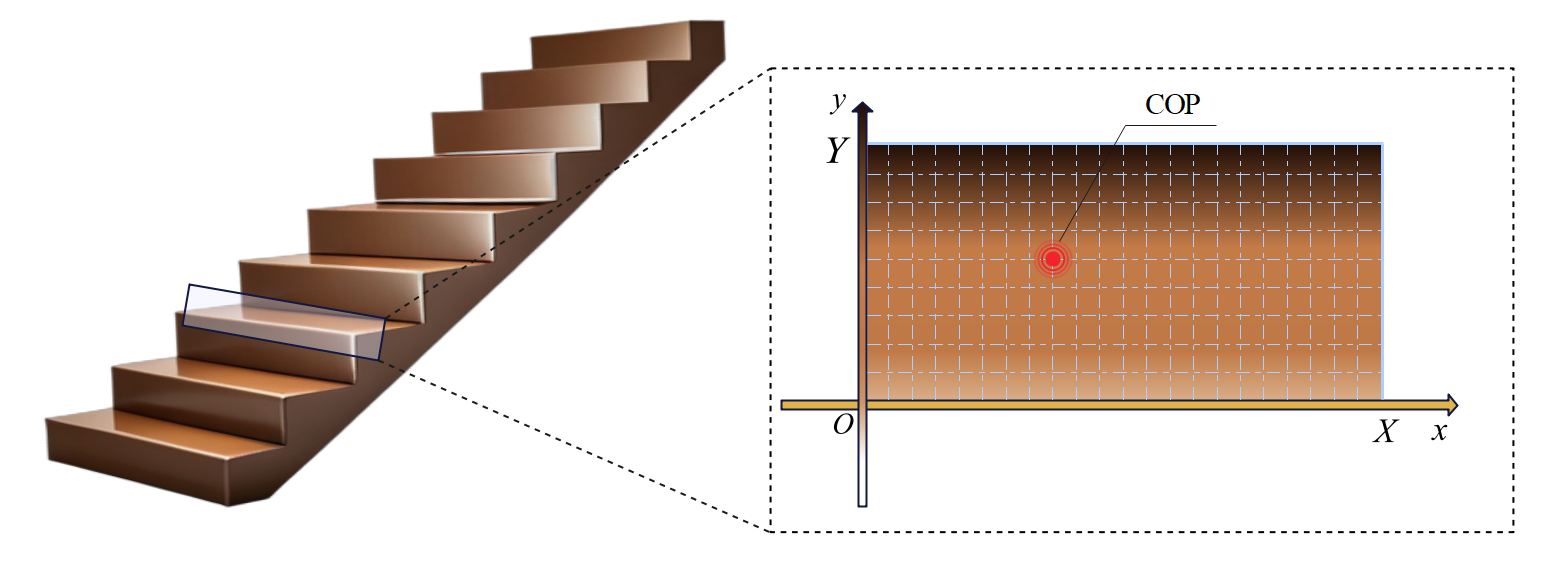
\includegraphics[width=0.9\linewidth]{美赛Latex模板/image.png}
	\caption{Rasterized diagram of the stair surface}
	\label{Rasterization}
     \vspace{-2em} % 用来调间距
\end{figure}

The COP[] is defined as the center of each grid.
\begin{equation}
     x=\lfloor \frac{p}{G_s} \lfloor\quad,\quad y=\lfloor \frac{G_s}{Y}\lfloorx = \left\lfloor \frac{p}{G_s} \right\rfloor \quad,\quad y = \left\lfloor \frac{G_s}{Y} \right\rfloor
\end{equation}
w$p$ is the distance from this COP to the leftmost side of the step, $q$ is the distance from this COR to the bottom edge of the step, and $G_s$ is the size of the grid. Denote the amount of wear at grid COP(x,y) as $d(x,y)$. The archaeologist measures the wear volume of the stone steps and then constructs the actual wear matrix $D^{measure}(x,y)$.
\subsubsection{Wear Volumn Model}
Wear results from behavior over time for a material as hard as stone. The total number of steps taken on the same spot determines the amount of wear on that spot. The length of time determines the time scale of cumulative wear. The hardness and abrasion resistance of the material directly affects the wear rate. In addition, different distributions of steps and applied gravity in different areas can lead to uneven wear. In order to accurately obtain information about the steps, we introduced a comprehensive Wear Volume Model, combining the wear distribution model with the introduction of time, material, and number of footsteps:
\begin{equation}
    d(x,y) = T\cdot{N_d}\cdot{D(x,y)}\cdot{G}\cdot{k_m}
\end{equation}
\label{equation3.2}
$d(x,y)$ represents the data measured by the archaeologist, $T$ denotes the number of days, $N_d$ indicates the average number of people who walked the stairs each day, $D(x,y)$ is the wear distribution function, we discuss it in Section 3.2. $G$ is the average gravitational force exerted on those who walked the stairs, and $k_m$ is defined as the wear volume coefficient (the amount of wear and tear per unit of $N$ on the stone steps). Further, we analyze the parameters $k_m$ and $G$.
\begin{itemize}
	\setlength{\parsep}{0ex} %段落间距
	\setlength{\topsep}{2ex} %列表到上下文的垂直距离
	\setlength{\itemsep}{1ex} %条目间距
	\item \textbf{Archard wear theory ($k_m$)} \\
\quad Archard wear theory is one of the classical wear models, proposed by J.F. Archard. The theory is used to describe the wear behavior of solid surfaces. Each step exerts a certain positive pressure on the step in the process, which can be directly applied to analyze the wear suffered by the step surface. At the same time, although the relative motion distance between the person and the step during walking is limited, the slight sliding of each step will cause localized wear on the step surface. Therefore, Archard's wear theory is applicable to analyze the wear of steps caused by people walking. The theory defines the basic formula for the unit wear coefficient of a solid $k_m$, which is specified as:
\begin{equation}
    k_m = K\cdot{\frac{d}{H}}
\end{equation}
where $K$ denotes the stone wear coefficient, $d$ represents the relative sliding distance of the tread surface, and $H$ indicates the material hardness of the stone. Based on the site survey, an information review is needed to obtain $K$ and $H$.

   \item \textbf{Gravity Assessment Model ($G$)}\\
   \quad The same step may be used by people of different ages and genders with different weight characteristics. We categorize the population into six groups: male minors (mm), female minors (fm), adult males (am), adult females (af), older men (om), older women (ow). To make the results more precise, we use their weight expectation as $G$ in the model, which is calculated as follows:
    \begin{equation}
        G=\sum_{i}u_i\cdot{p_i}
    \end{equation}
    \quad where $u_i$ describes the average weight of each population, $p_i$ indicates the proportion of each population to the total population. If the archaeologists have the information on the local age and gender structure, they can fill in the corresponding proportions to obtain a more localized weight expectation $G$. This can make the calculation results more accurate and increase the flexibility of the model.
    
    \quad If they don't have, based on the global weight data provided by the XXX Bureau of Investigation, we give data as a reference, which is shown in Table.
\end{itemize}

Integrating \autoref{equation3.2}, we obtain the expression for the average wear $d_{avg}$ as
\begin{equation}
    d_{avg} = \frac{1}{A_{ceff}}\int_{A_{ceff}} T\cdot{N_d}\cdot{D(x,y)}\cdot{G}\cdot{k_m}dxdy
\end{equation}
in this equation, $A_{ceff}$ denotes the area of the steps overlook.

\subsubsection{Calculation of Age and Frequency of Stone Steps}
According to the analysis above, When $D$,$G$, and $k_m$ are determined,  the stone steps' age $T$ and frequency of use $N_d$ can be solved for each other. The specific formulas are shown below:
\begin{equation}
    T = \frac{A_{ceff}\cdot{d_{avg}}}{N_d\cdot{G}\cdot{k_m}}
\end{equation}
\begin{equation}
    N_d = \frac{A_{ceff}\cdot{d_{avg}}}{T\cdot{G}\cdot{k_m}}
\end{equation}
At this point, the stone steps' age $T$ and frequency of use $N_d$ can be sought.

\subsection{Wear Distribution Model}
Each step on the steps can be regarded as obeying independently and identically distributed. Research shows a linear relationship between the number of steps and the amount of wear, and only when the cumulative number of steps reaches a large size, significant wear on the surface of the step stone can be produced.  According to the \textbf{Central Limit Theorem}, when the number of independent random samples is large enough, even if the original distribution is not normal, the distribution of the sample mean will converge to the normal distribution. Therefore, when the sample size is large, the cumulative distribution of steps tends to be normal, and the cumulative wear will also be normal.

Since there is no significant correlation between the lateral and longitudinal positions of the footsteps on the stone stairs, the cumulative wear of pedestrians at each position in both the x- and y-directions can be described as a superposition of normal or multi-normal distributions when the number of steps is sufficiently high. And the distributions reflect the traffic patterns of people on that set of stairs.
\subsubsection{Wear Distribution in the Y-direction - Judging the Direction}
Studies of the gait cycle show that during stair ascent, the first peak appears in the heel, while during stair descent, the first peak is in the forefoot. This is shown in Figure(). In addition, observing people's daily stair movement behavior, it is found that pedestrians' point of impact is closer to the lower edge of the steps when going up the stairs than when going down the stairs. 
\begin{figure}[H]
\vspace{-1.0em}
	\centering    
	\subfigure[stair ascent]{				% 图片1([]内为子图标题)
		\label{fig:showup}							% 子图1的标签
		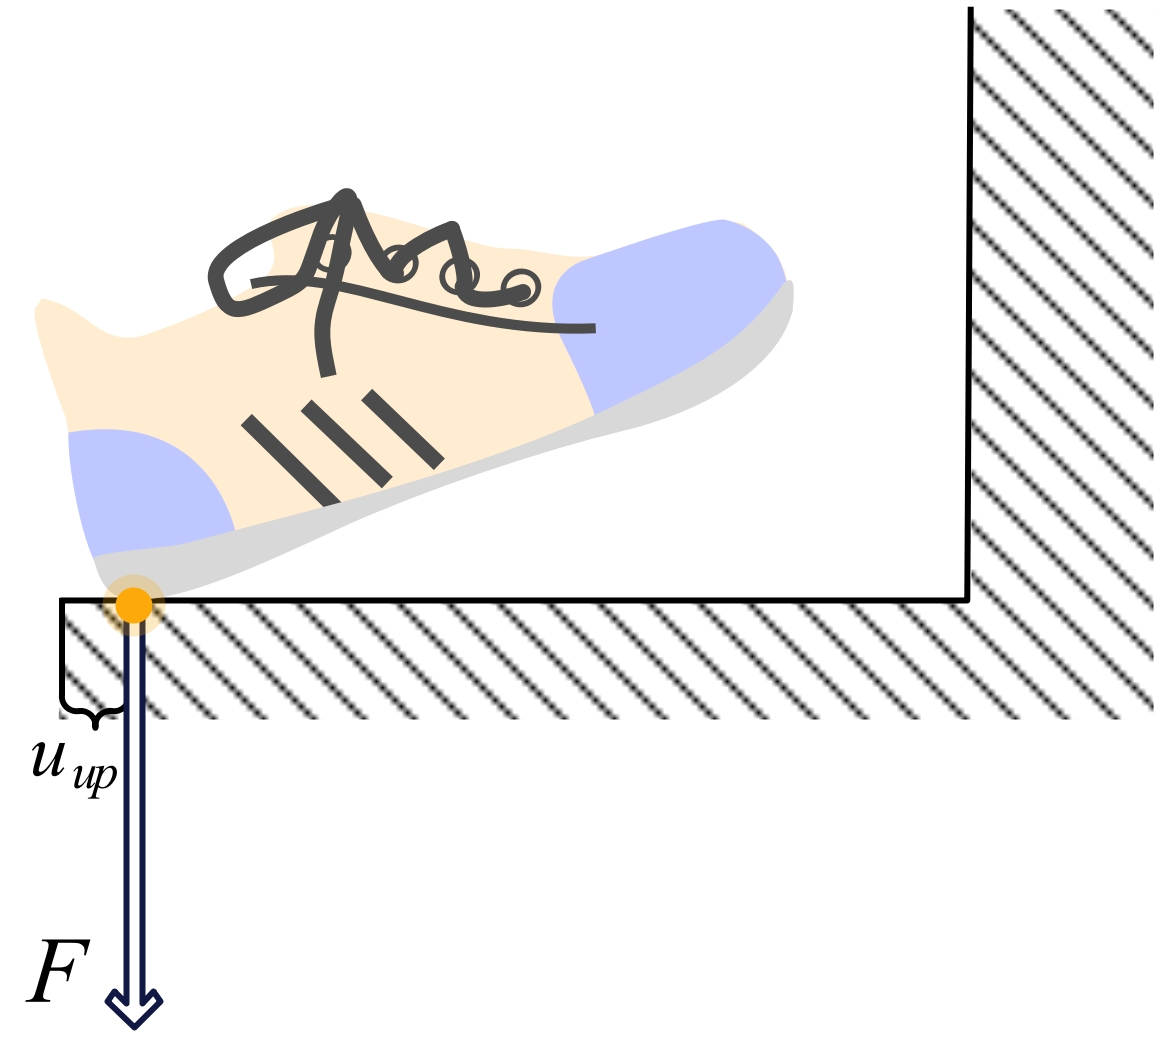
\includegraphics[width=0.4\textwidth]{美赛Latex模板/shoeUp.jpg}}% 子图1的相对位置
	\subfigure[stair descent]{				% 图片2
		\label{fig:showDown}						% 子图2的标签
		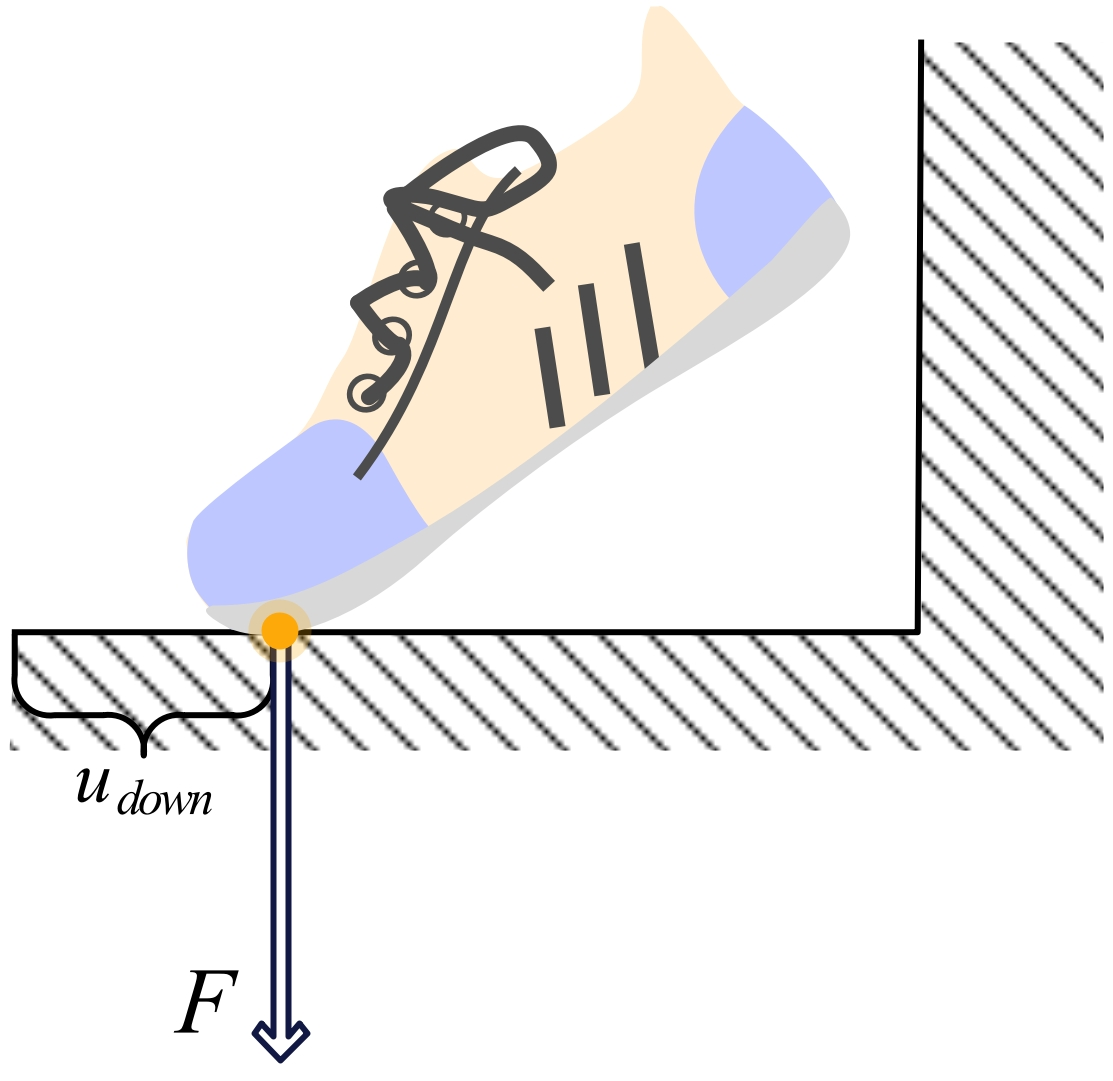
\includegraphics[width=0.4\textwidth]{美赛Latex模板/shoeDown.jpg}}% 子图2的相对位置
	\caption{Force diagram of walking}		% 总图标题
	\label{fig:ForceDiagram}									% 总图标签
    \vspace{-1.0em}
\end{figure}

With the conclusion above, we can judge whether people using the stairs favored a certain direction of travel based on the wear distribution of y-direction. 

\begin{figure}[H]
\vspace{-1.0em}
	\centering    
	\subfigure[Upward direction - Wear Distribution]{				% 图片1([]内为子图标题)
		\label{fig:upa}							% 子图1的标签
		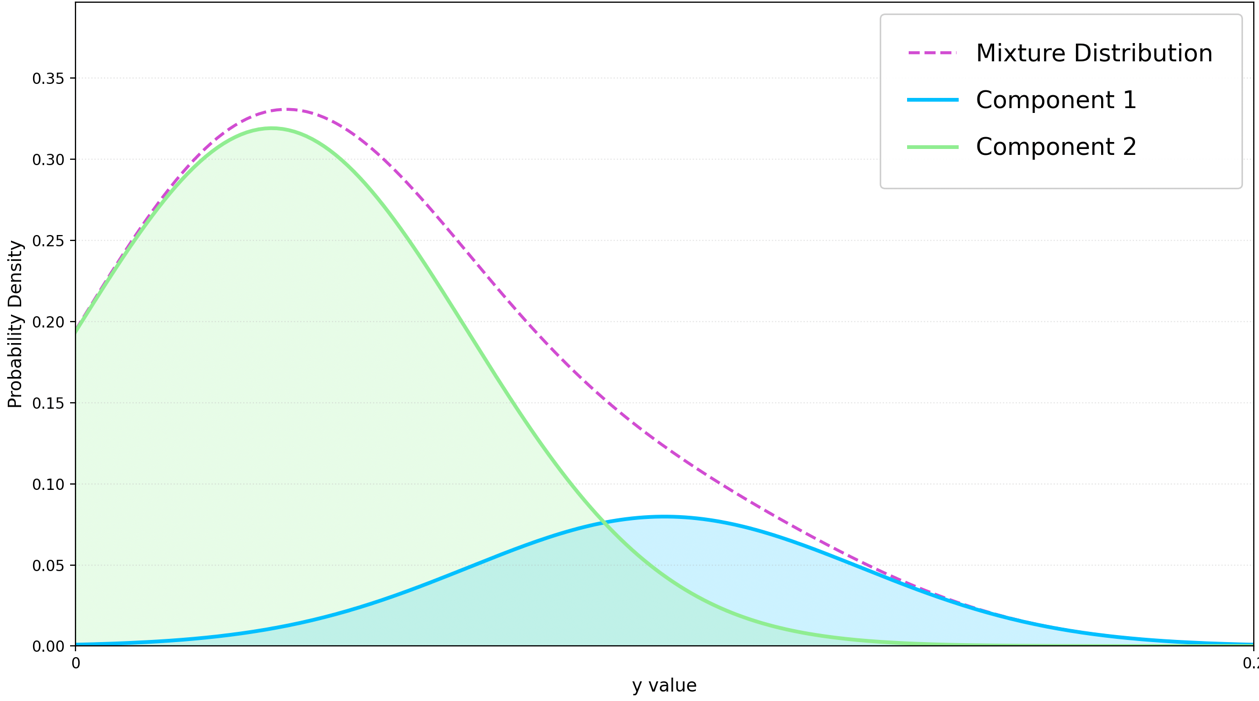
\includegraphics[width=0.5\textwidth]{美赛Latex模板/upward.png}}% 子图1的相对位置
	\subfigure[Upward direction]{				% 图片2
		\label{fig:upb}						% 子图2的标签
		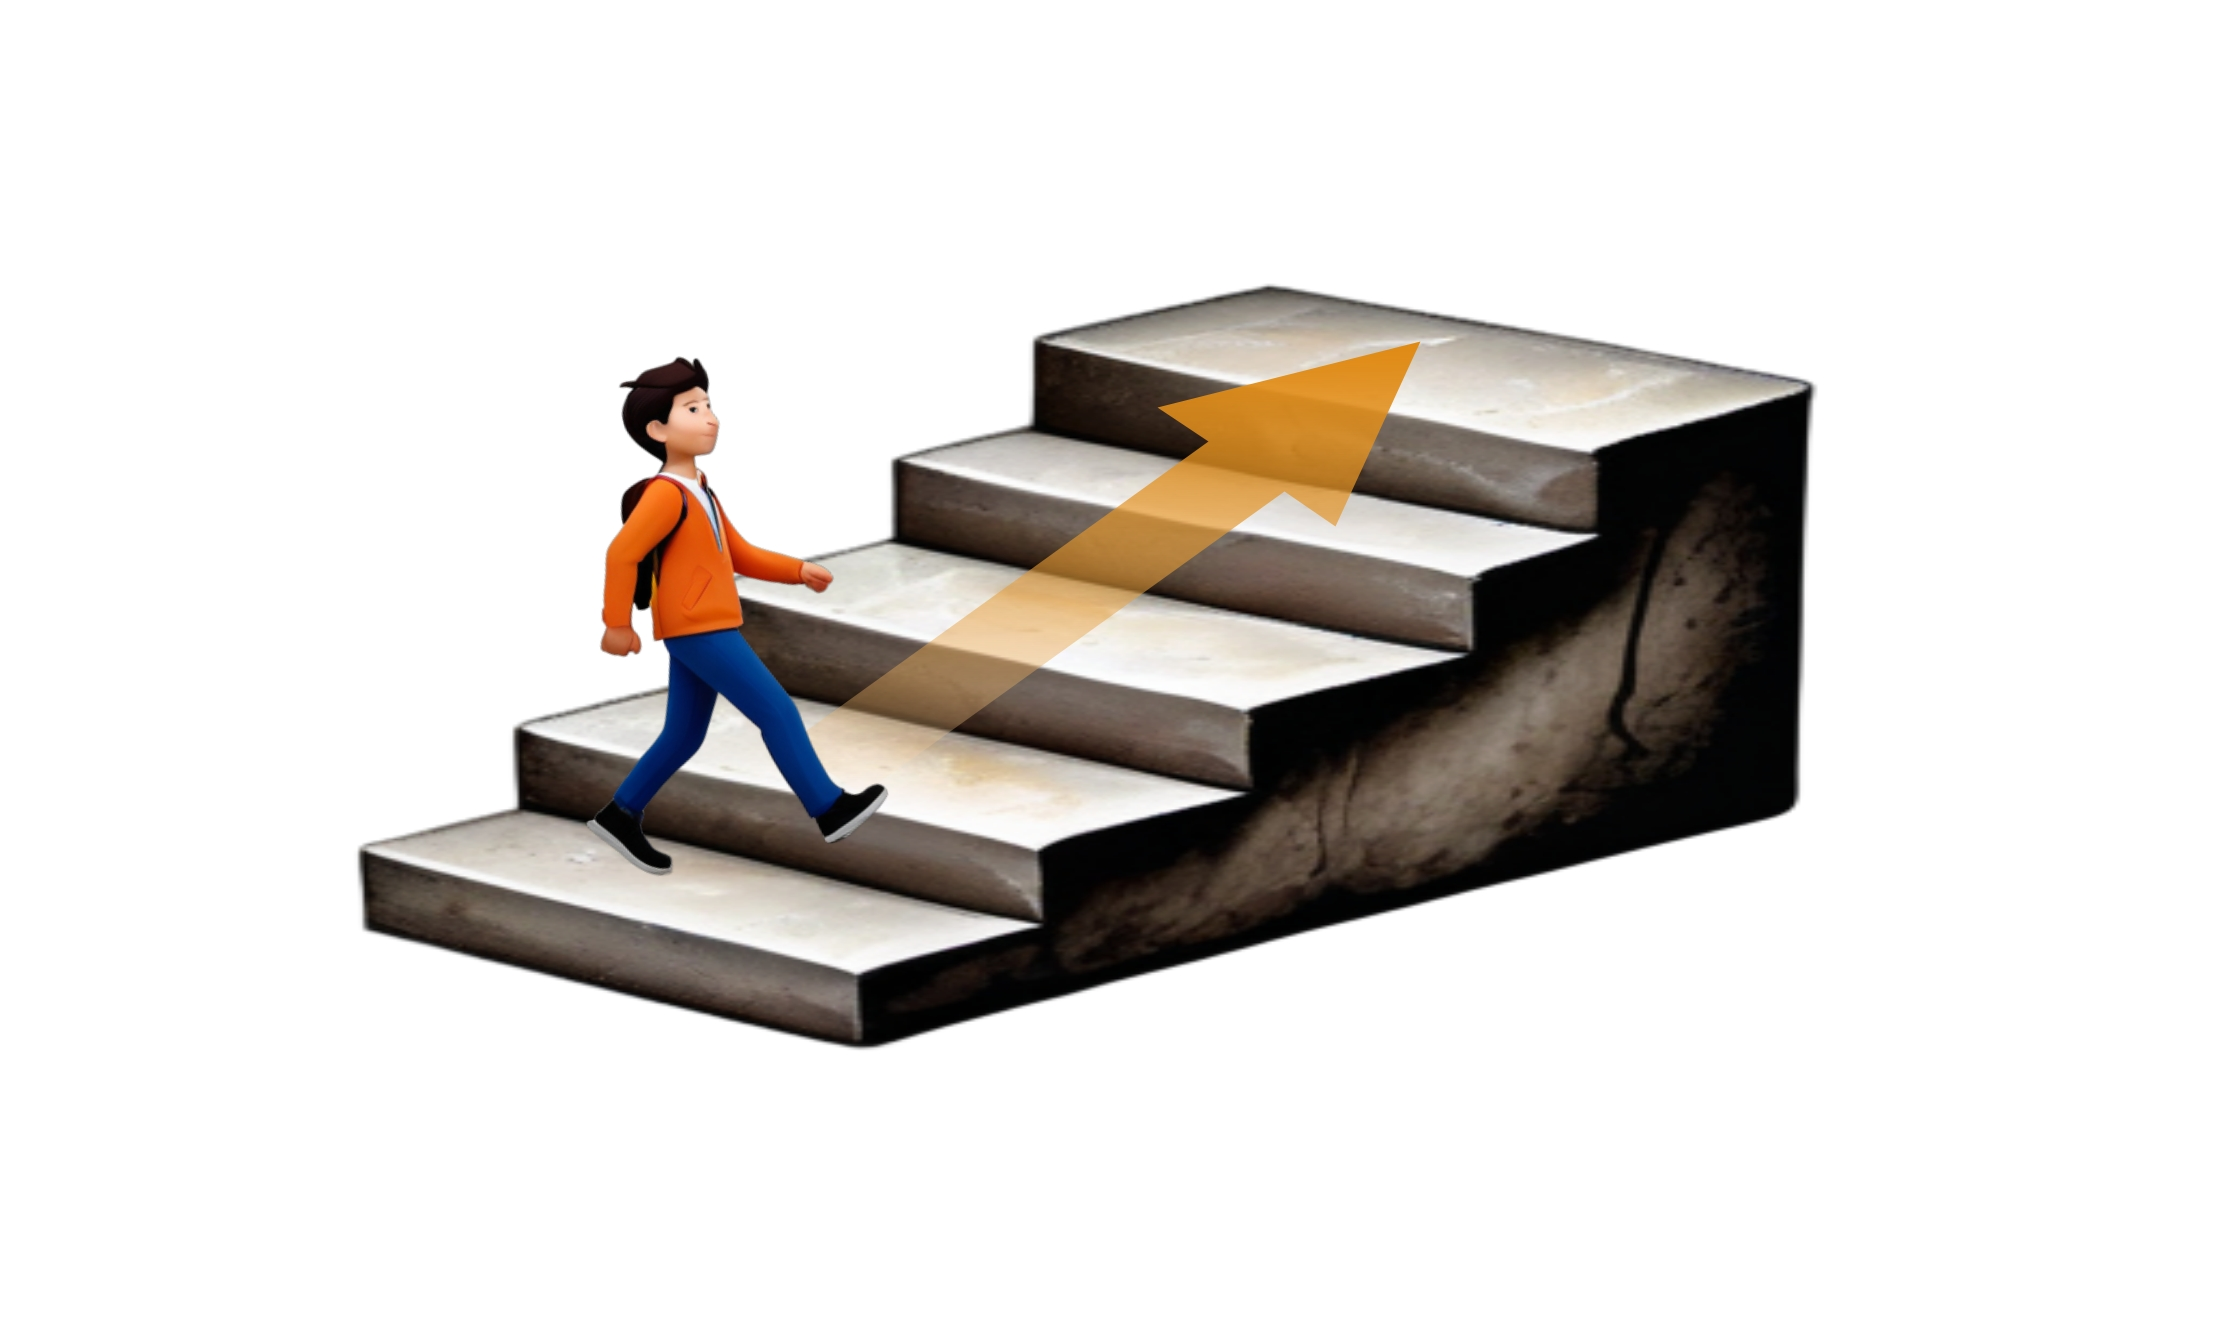
\includegraphics[width=0.5\textwidth]{美赛Latex模板/单行.jpg}}% 子图2的相对位置
    \vspace{-1.0em}
    \\
    \subfigure[Double Direction - Wear Distribution]{				% 图片3([]内为子图标题)
		\label{fig:doua}							% 子图3的标签
		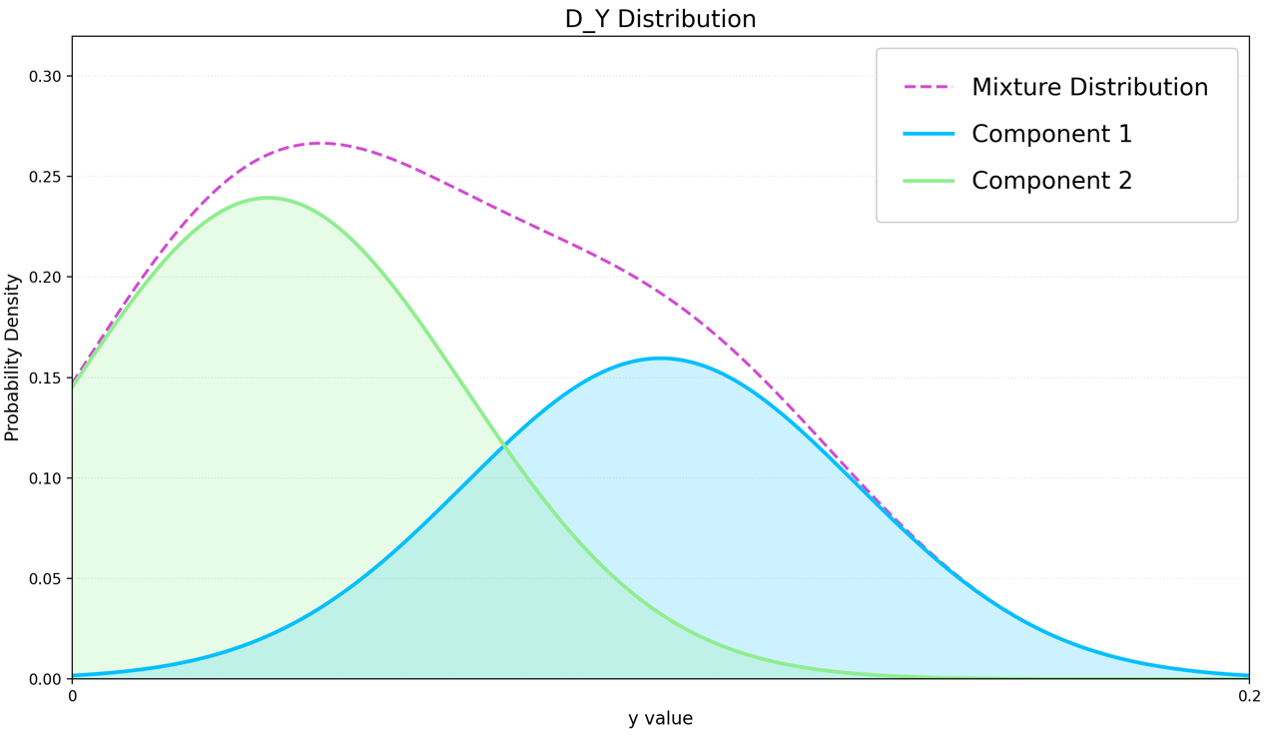
\includegraphics[width=0.5\textwidth]{美赛Latex模板/doubledirection.png}}% 子图3的相对位置
	\subfigure[Double Direction]{				% 图片4
		\label{fig:doub}						% 子图4的标签
		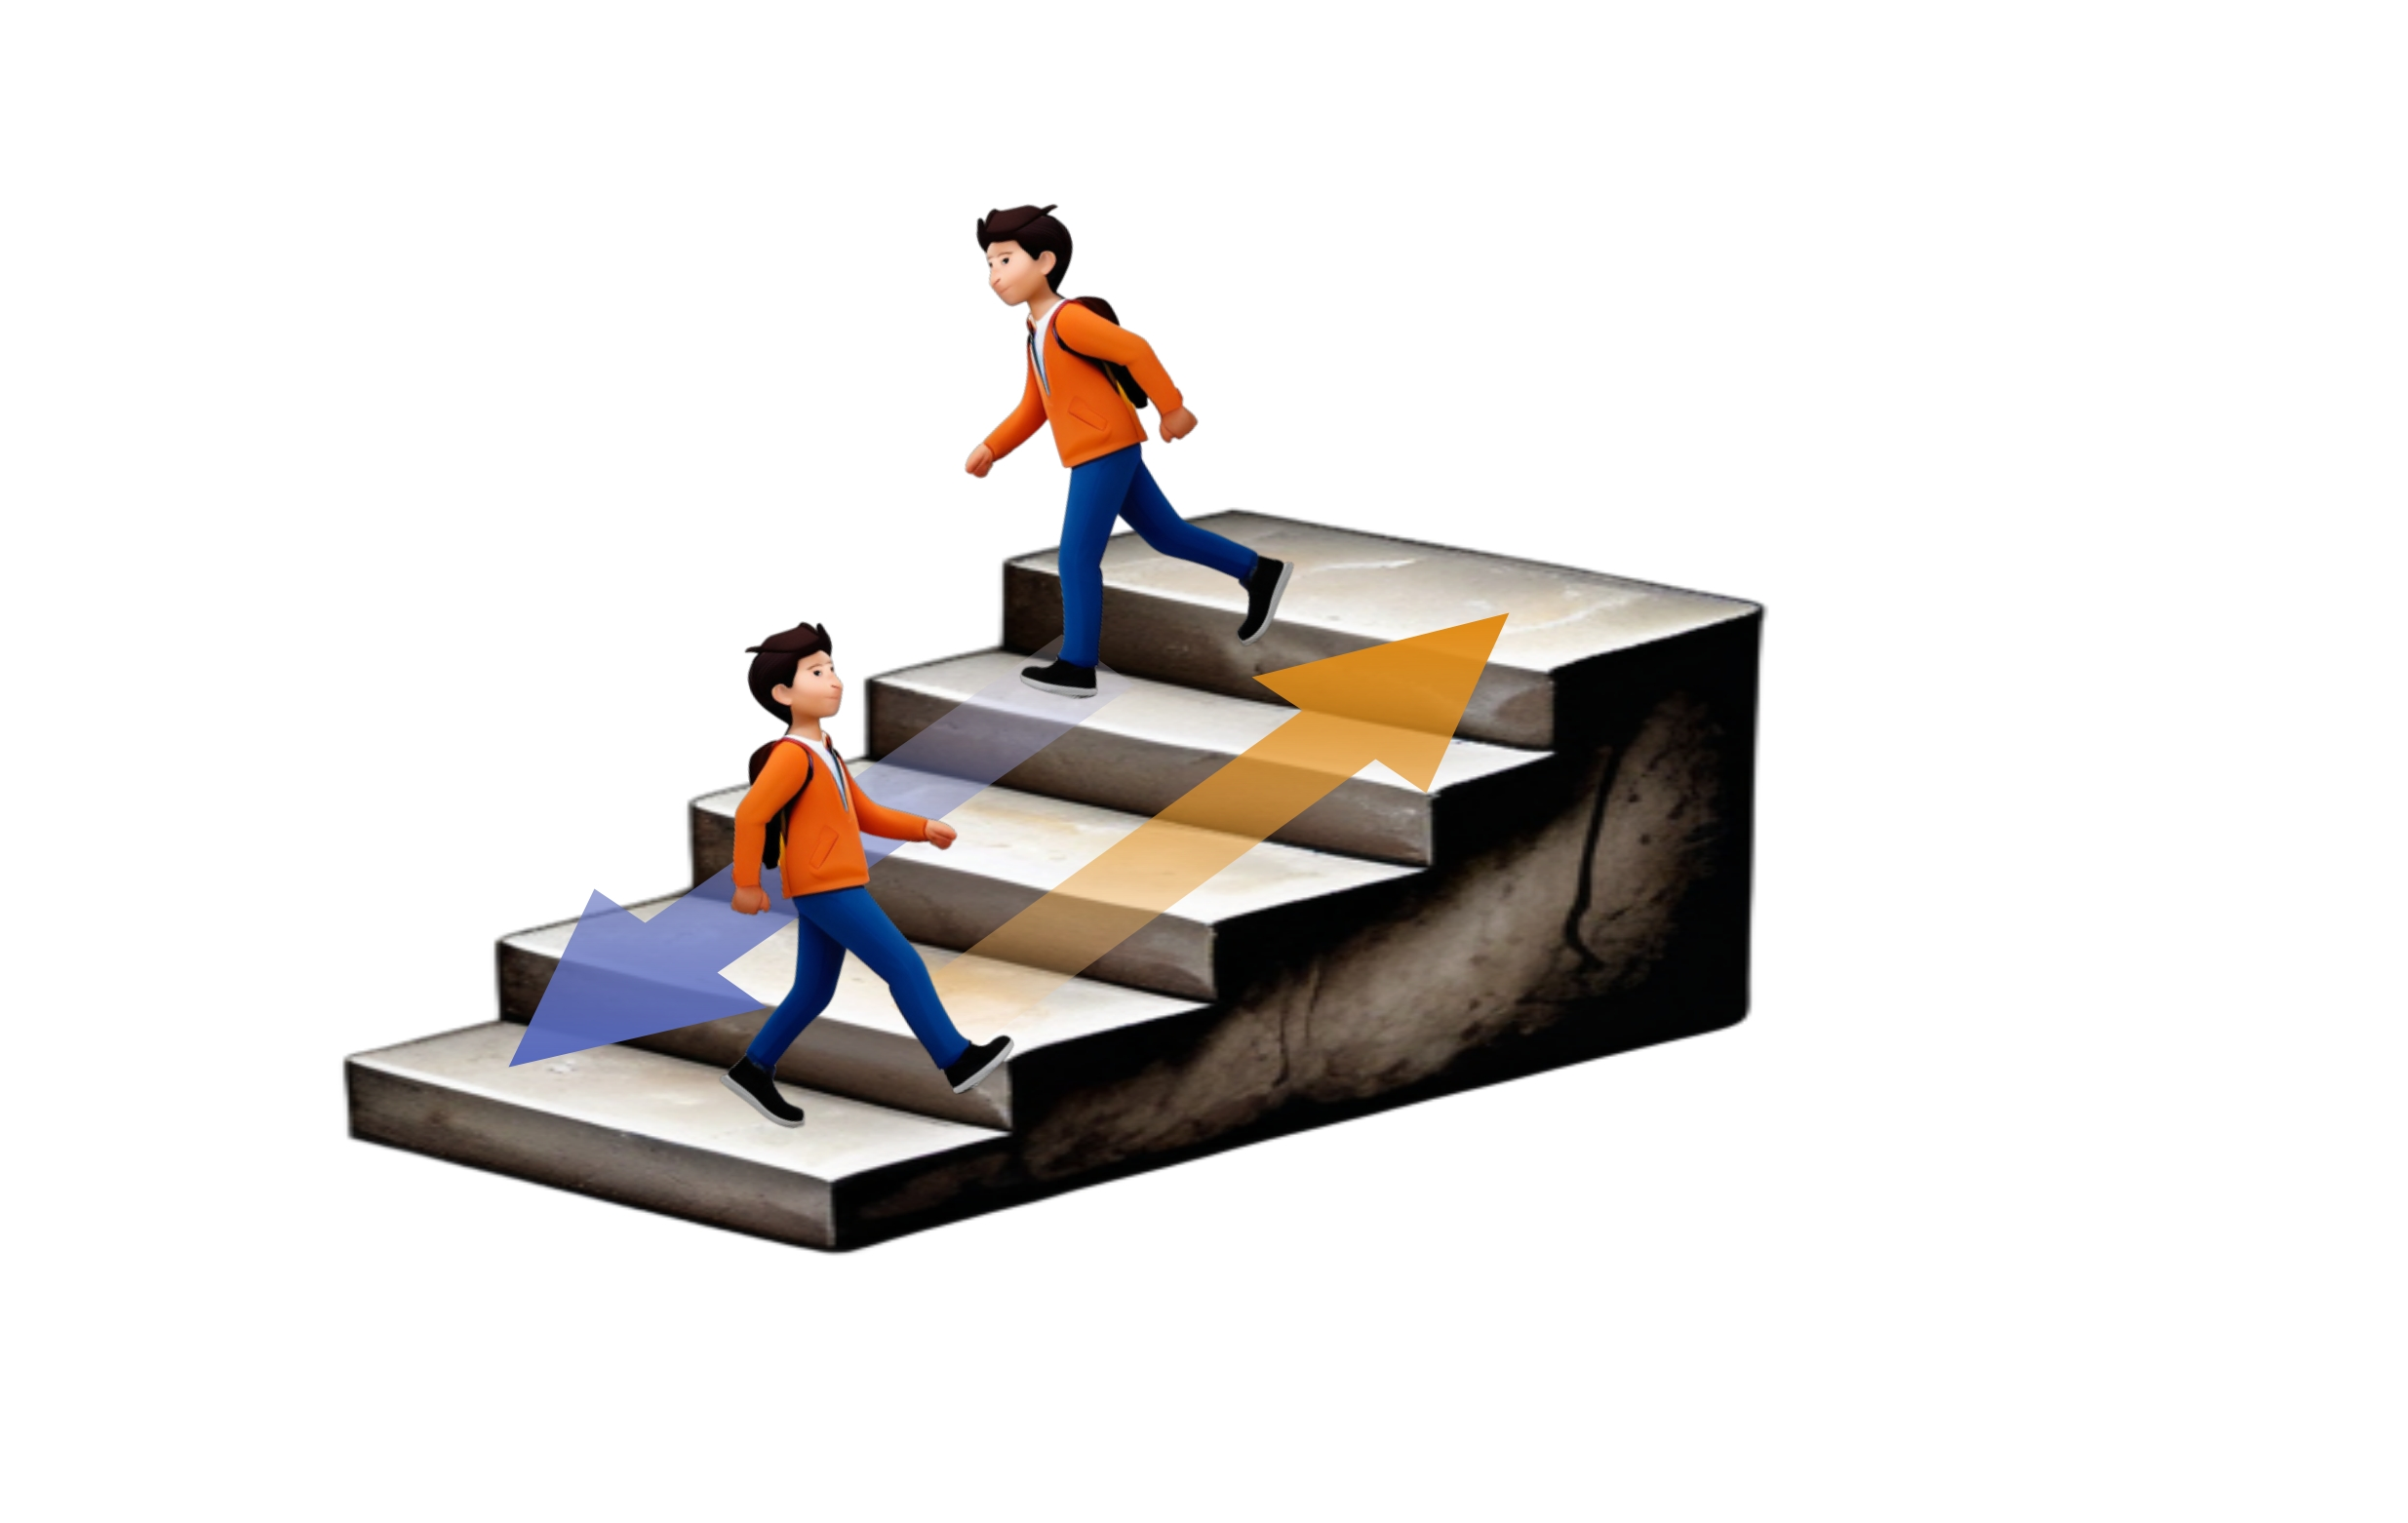
\includegraphics[width=0.5\textwidth]{美赛Latex模板/双向通行.jpg}}% 子图4的相对位置
	\caption{Distribution of wear in the Y-direction and the corresponding number of people}		% 总图标题
	\label{fig:Y-two}									% 总图标签
    \vspace{-1.0em}
\end{figure}

As shown in \autoref{fig:Y-three},  there are two peaks, which means that the marginal distribution in the y-direction is a superposition of two normal distributions. This indicates that stairs were usually used in both directions. The number of people traveling up and down the stairs can be compared based on the size of the peaks. Similarly, one peak demonstrates that people using the stairs favored a certain direction of travel. If the y-value at the peak is small, people favored upward travel. If it is larger, downward travel was favored.


We further quantify the results so that archaeologists can determine the direction and the proportion of up-and-down people more intuitively. Using knowledge of probability statistics, we construct the distribution of wear in the Y-direction:
\begin{equation}
D_{y}\sim w_{up}\cdot N_i(\mu_{up},\sigma_{up})+w_{down}\cdot N_i(\mu_{down},\sigma_{down})
\end{equation}
$w_{up}$ denotes the ratio of people going up to the total number of people, while $w_{down}$ denotes the ratio of people going down to the total number of people. $mu_{up}$ is the distance between the center of the stepping surface of the person going up and the outermost part of the stone step, and $mu_{down}$ is the distance between the center of the stepping surface of the person going down and the outermost part of the stone step. $sigma_{up}$ describes the degree of longitudinal dispersion of people going upstairs, and $sigma_{down}$ describes the degree of vertical dispersion downstairs. 
\subsubsection{Wear Distribution in the X-direction - Calculating the Number of Parallels}
When people walk on the stairs in a single-step strategy, the peaks of the normal distribution in the x-direction of the steps describe the main concentration area of pedestrians. And the number of peaks reflects the lateral distribution characteristics of pedestrians on the road. We describe the wear distribution in this direction as:
\begin{equation}
    D_{x}\sim w_i\sum_{i}N_i(\sigma_i,\mu_i)
\end{equation}
$n$ represents the number of parallel lanes on the same step of the stone staircase, $w_i$ is the ratio of the number of people in the lane $i$ to the total number of people,  $\mu_i$ denotes the distance of the center of the lane $i$ from the leftmost end of the stone staircase, and $\sigma_i$ indicates the degree of lateral dispersion of lane $i$.

\begin{figure}[H]
\vspace{-1.0em}
	\centering    
	\subfigure[Travel single - Wear distribution]{				% 图片1([]内为子图标题)
		\label{fig:singlea}							% 子图1的标签
		\includegraphics[width=0.5\textwidth]{美赛Latex模板/01b1074bcc64cddb7d974a410b9787d4.png}}% 子图1的相对位置
	\subfigure[Travel single]{				% 图片2
		\label{fig:singleb}						% 子图2的标签
		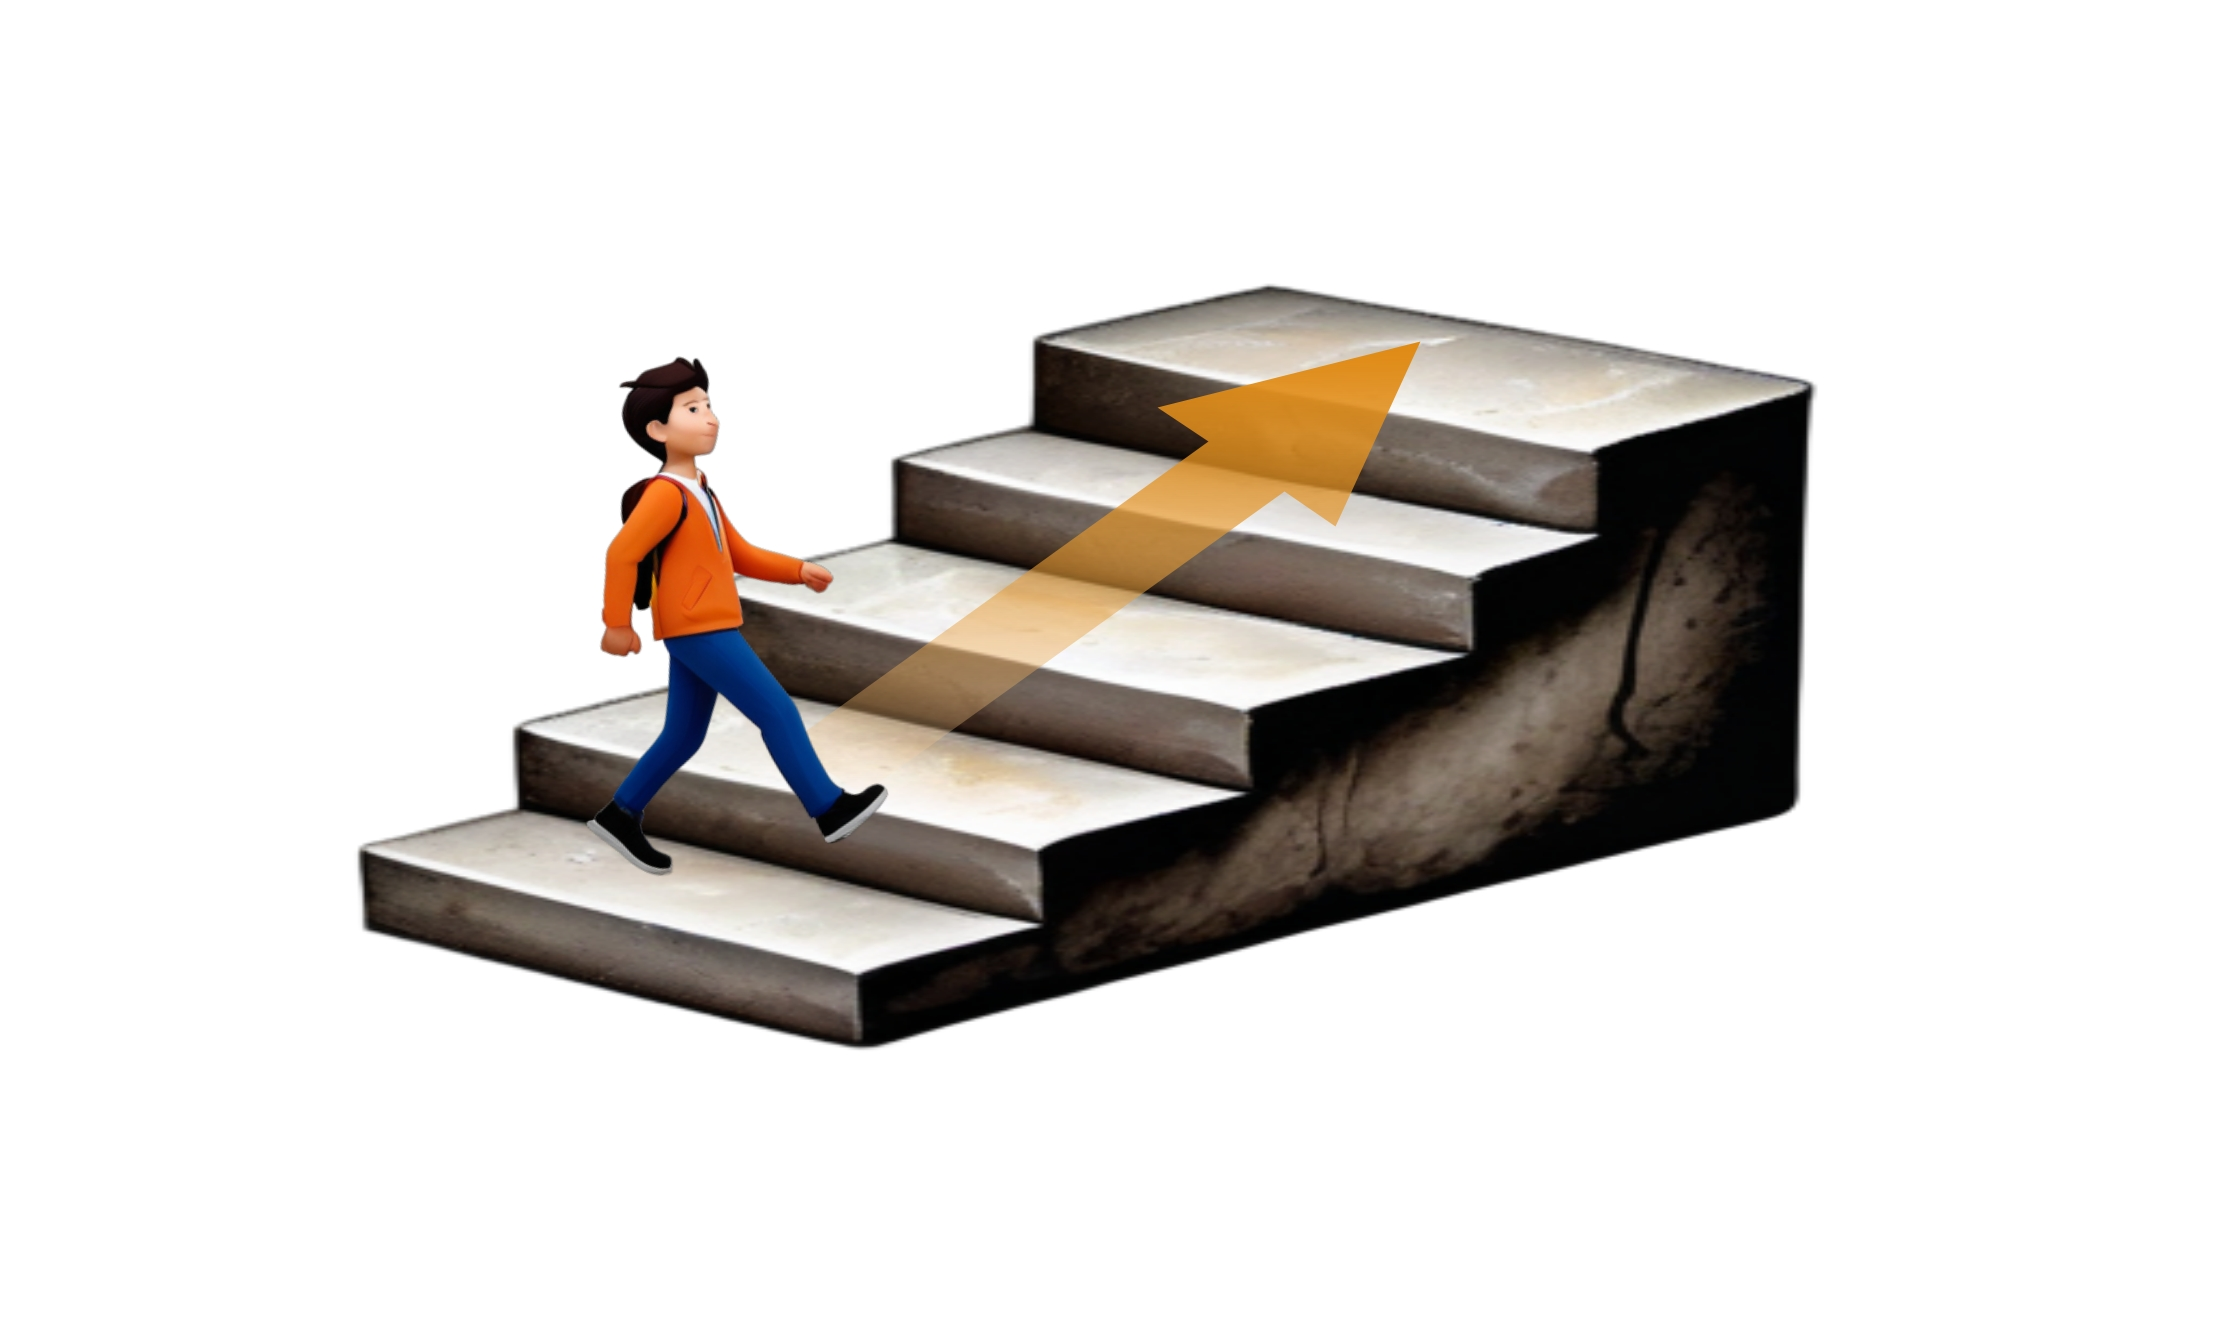
\includegraphics[width=0.5\textwidth]{美赛Latex模板/单行.jpg}}% 子图2的相对位置
    \vspace{-1.0em}
    \\
    \subfigure[Side by side - Wear distribution]{				% 图片3([]内为子图标题)
		\label{fig:twoa}							% 子图3的标签
		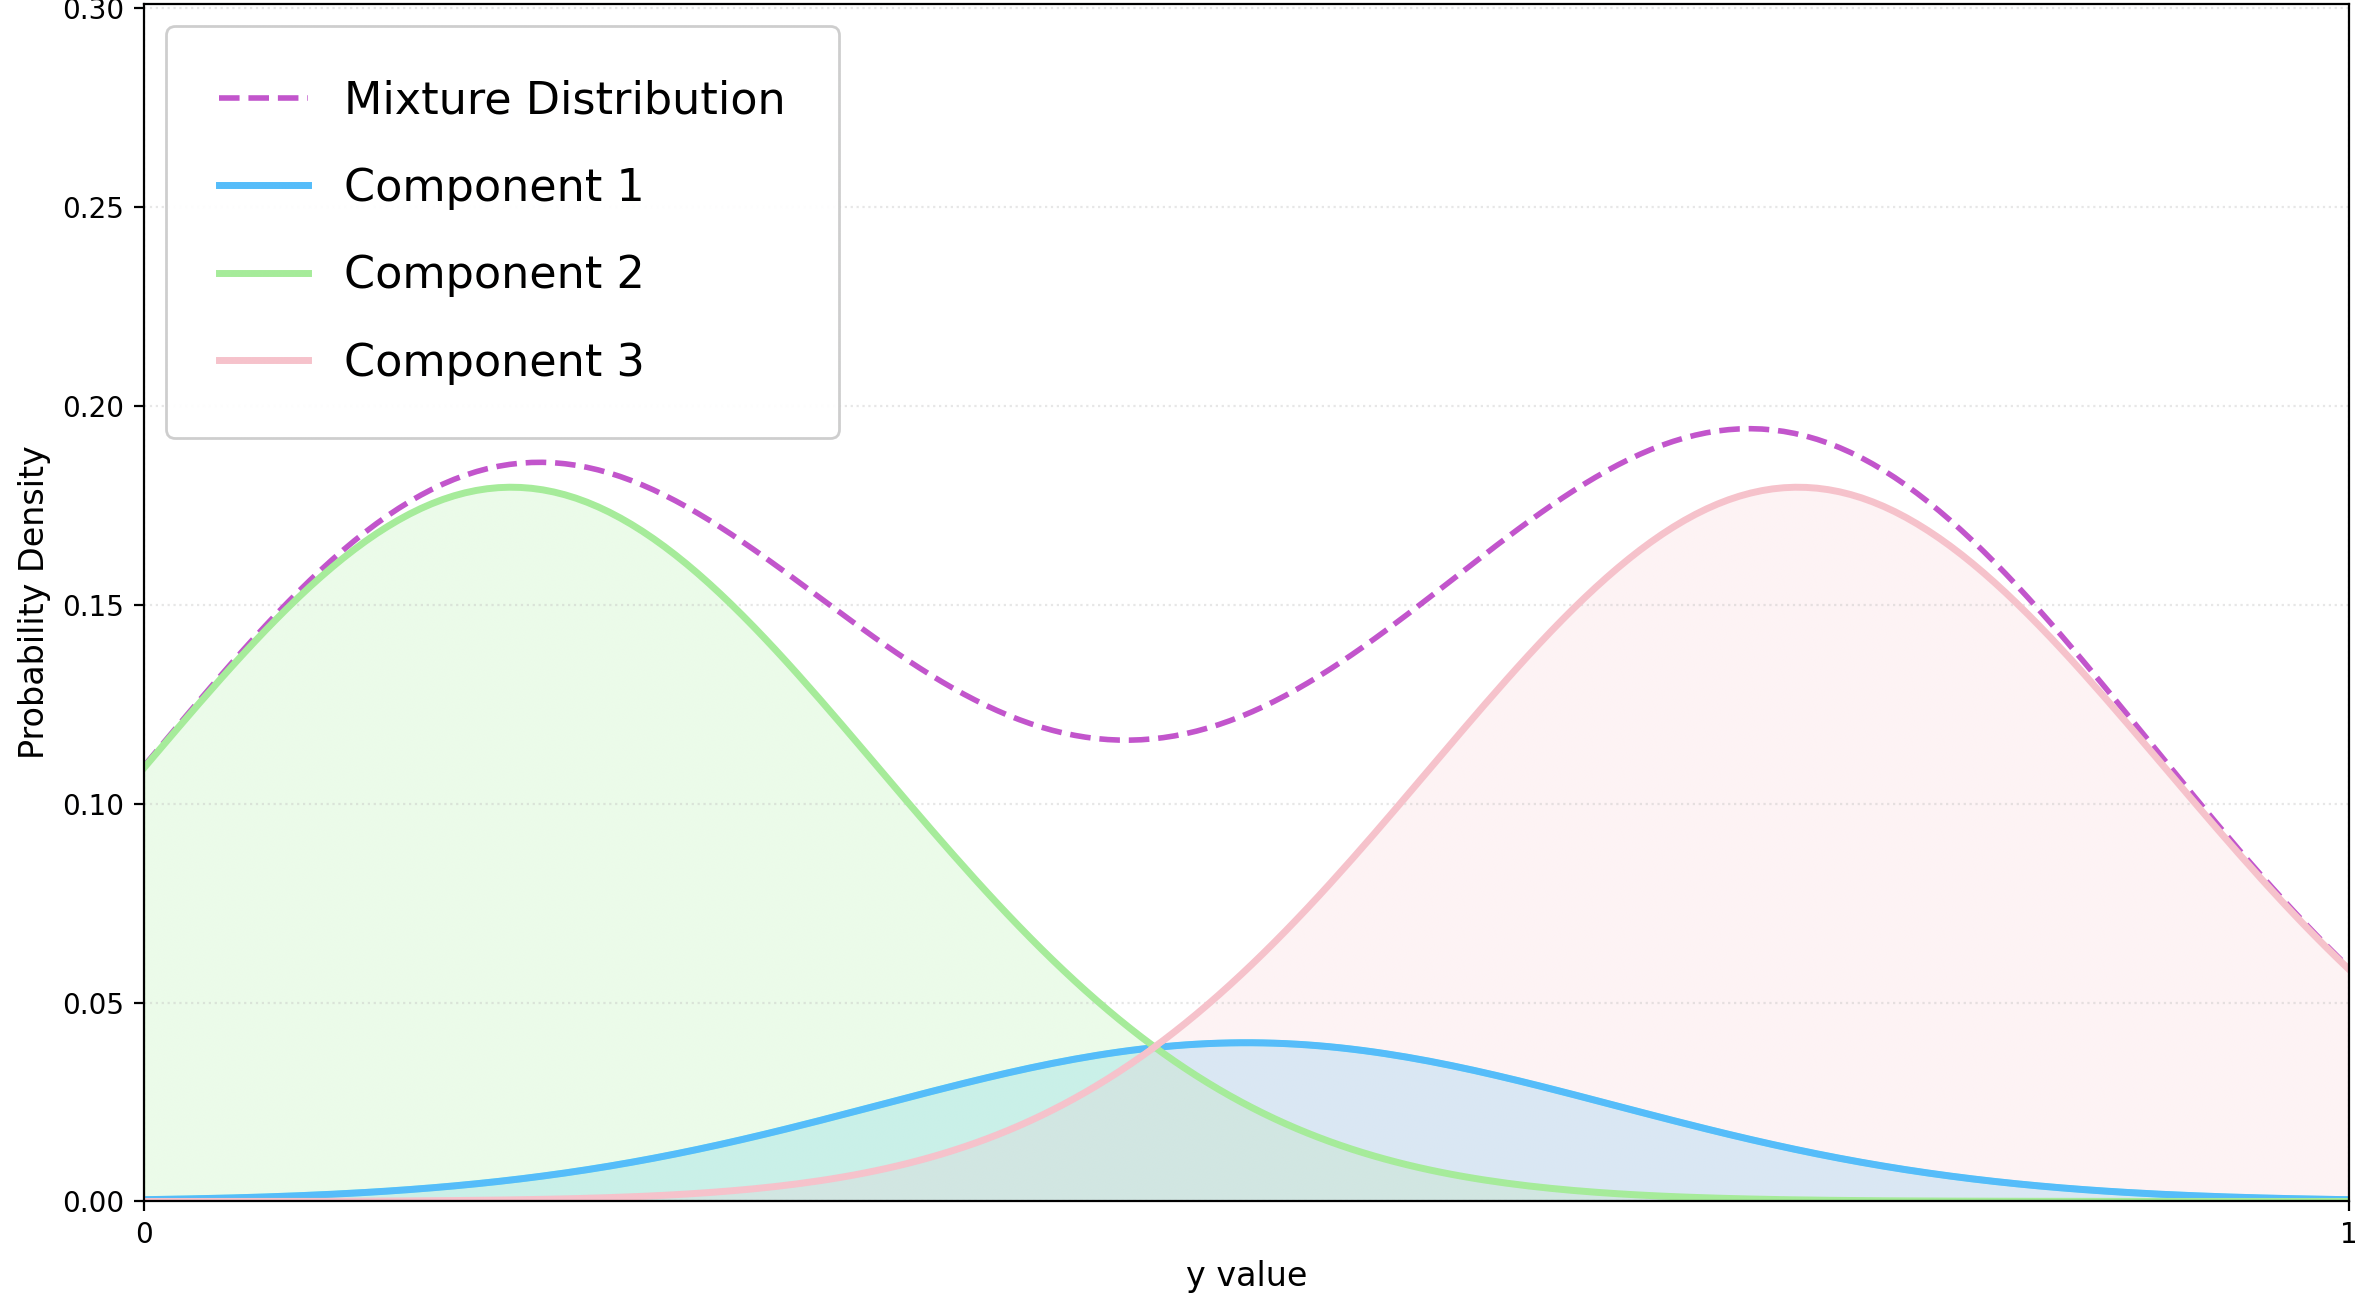
\includegraphics[width=0.5\textwidth]{美赛Latex模板/2people.png}}% 子图3的相对位置
	\subfigure[Side by side]{				% 图片4
		\label{fig:twob}						% 子图4的标签
		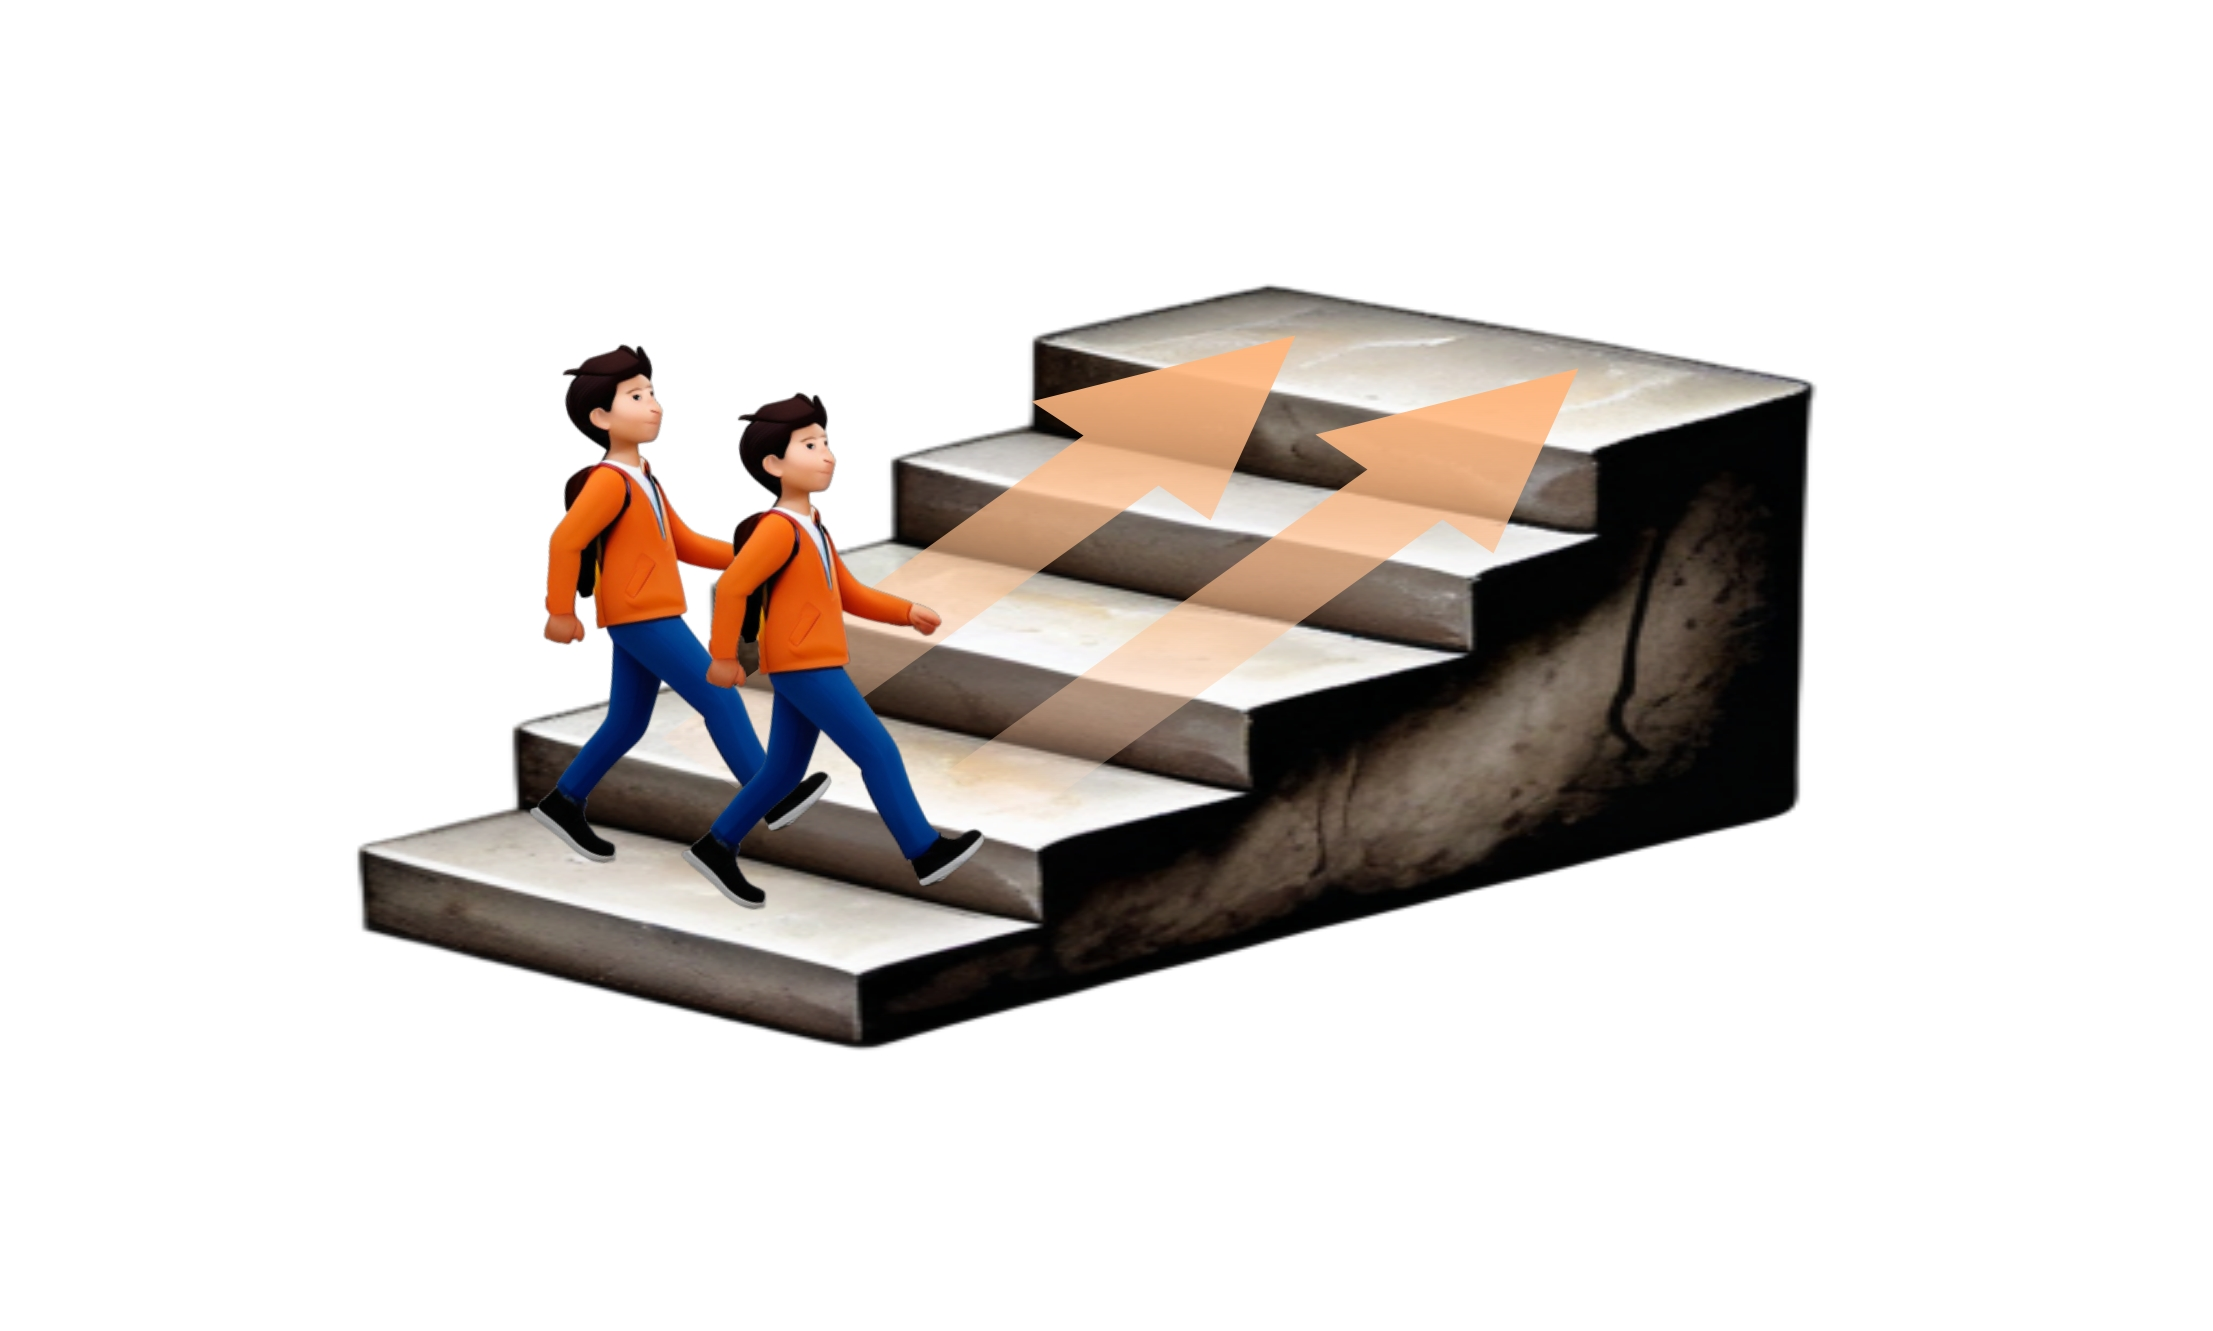
\includegraphics[width=0.5\textwidth]{美赛Latex模板/并行.jpg}}% 子图4的相对位置
	\caption{Distribution of wear in the X-direction and the corresponding number of people}		% 总图标题
	\label{fig:Y-two}									% 总图标签
    \vspace{-1.0em}
\end{figure}

The distribution describes how many people used the stairs simultaneously. The number of peaks is the number of people in parallel. In \autoref{fig:X-two}, we give some possible results for archaeologists as a reference: 
\begin{enumerate}[\bfseries 1.]
	\setlength{\parsep}{0ex} %段落间距
	\setlength{\topsep}{-1ex} %列表到上下文的垂直距离
	\setlength{\itemsep}{0ex} %条目间距
	\item When $i=1$, there is only one peak in the x-direction. It can be concluded that people using this stair preferred traveling single files. 
	\item When there are two peaks in the x-direction($i=2$), pairs of people climb the stairs side-by-side.  
	%\item Some small peaks may appear in the results. We consider this to be caused by people walking at different times of the day. It is not considered to be generated in parallel.
\end{enumerate}
\subsubsection{Wear Distribution Model}
Since the lateral position of a footstep on a stone step is not significantly correlated with its longitudinal position, we consider the covariance matrix of the wear distribution to be a diagonal array. For a stone step, we model the wear distribution as follows:
\begin{equation}
    D(x,y)=D_X\cdot{D_Y}
\end{equation}

We compute the actual wear matrix $D^{measure(x,y)}$ obtained from the archaeologist's measurements. Then, we can get its marginal distribution function:
\begin{equation}
    D_X^{measure}(x)=\sum_y{D^{measure}(x,y)}
\end{equation}
\vspace{-1.0em}
\begin{equation}
    D_Y^{measure}(y)=\sum_x{D^{measure}(x,y)}
\end{equation}
With these two edge functions, we can fit $D_x$ and $D_y$, which will help archaeologists obtain relevant information, such as people's traffic patterns.
\subsection{Stair Wear Model}
\subsubsection{Parameters to be measured}
Archaeologists are needed to carry out non-destructive measurements and access information to obtain accurate information and implement the model's solution. We provide the necessary parameters and suggest some measurement methods. It Is shown in Table \ref{parametertable}:

\begin{table}[H]
    \centering
    \vspace{-1.0em}
    \caption{Parameter need to be measured}
    \vspace{-1.0em}
        \begin{figure}[H]
    	\centering
    	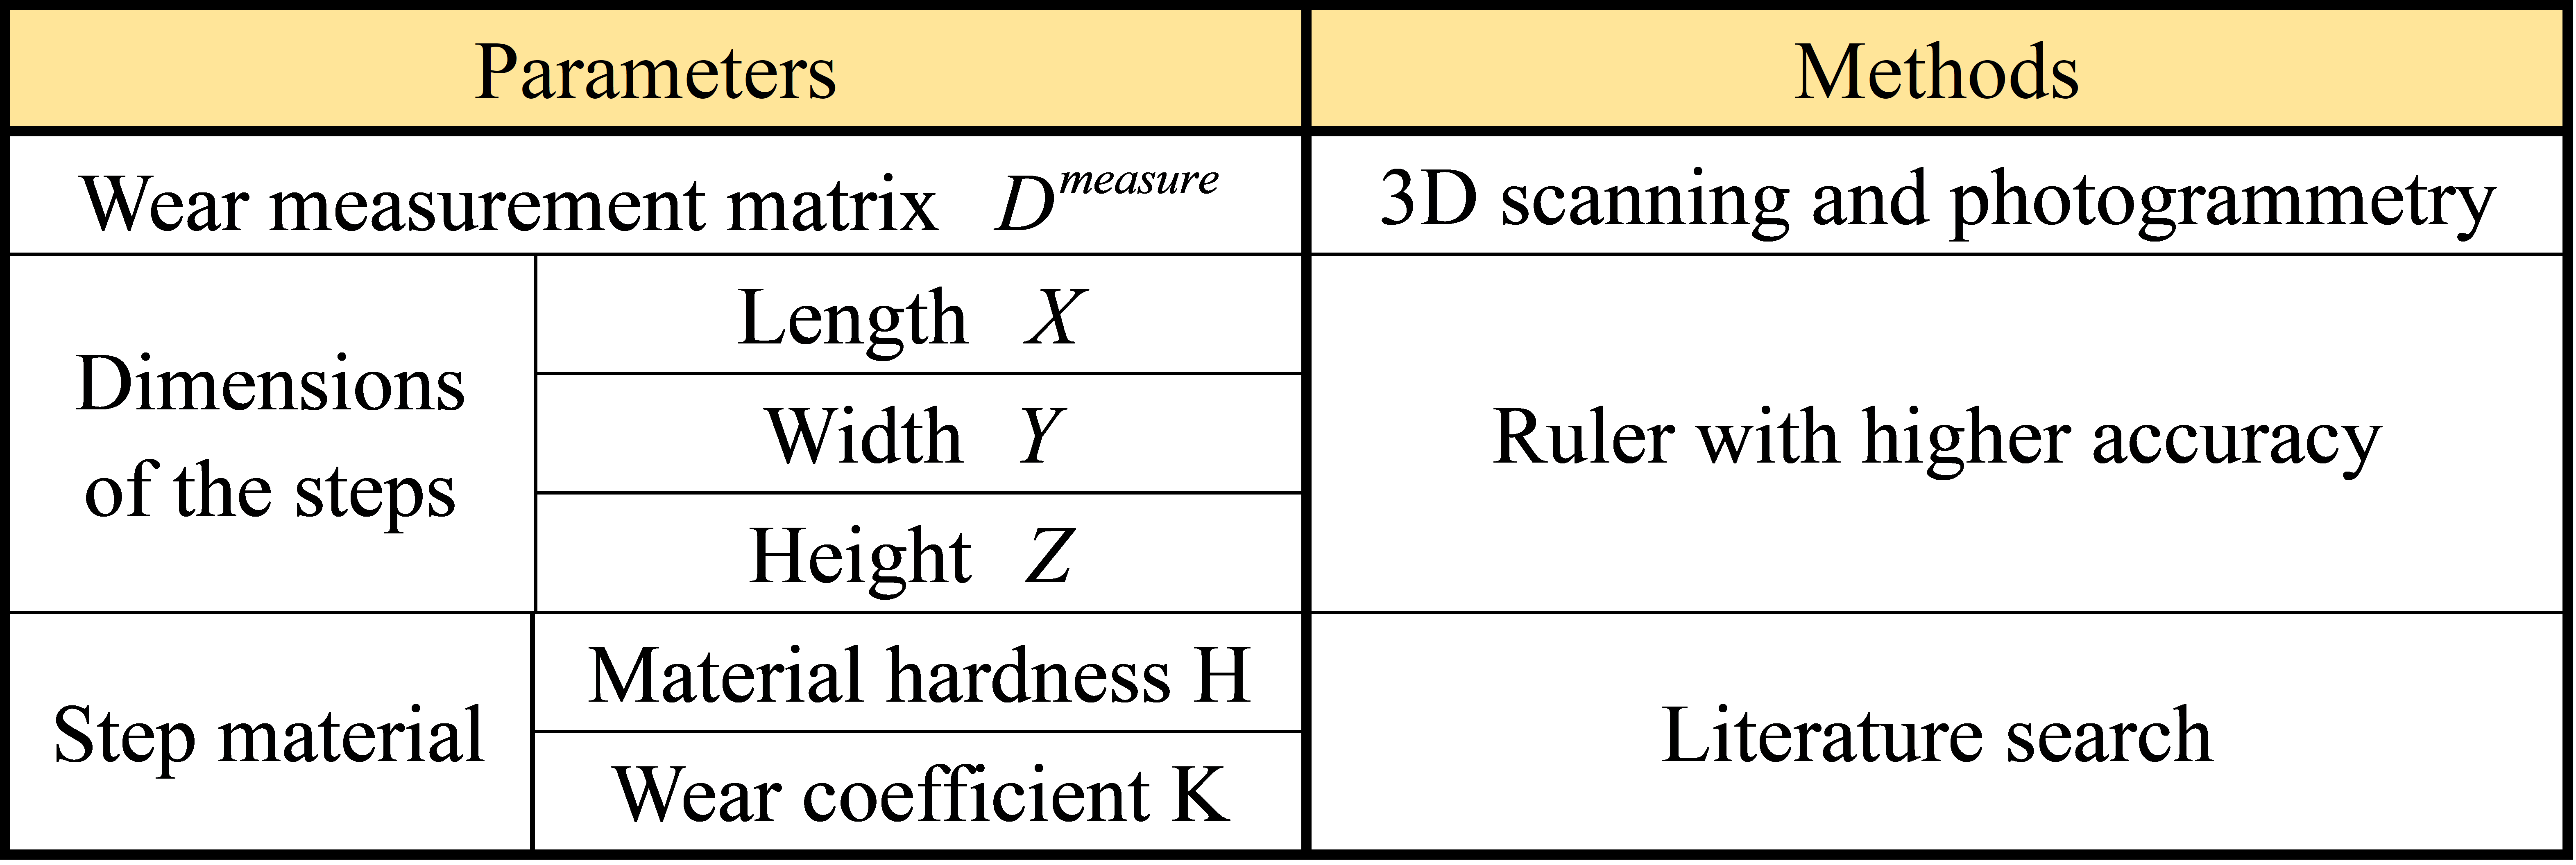
\includegraphics[width=0.8\linewidth]{美赛Latex模板/parametertable.png}
        \end{figure}
    \label{parametertable}
\end{table}


\vspace{-2.0em}
We all consider the methods that require minimum cost, fewer people, and the fewest tools.
\subsubsection{Overview of Stair Wear Model}
Based on the analysis above, the\textbf{ Stair Wear Model }is concluded as below:

\textbf{Wear Volume Model(WVM):}\\
\begin{equation}
\begin{aligned}
    & d_{avg} = \frac{1}{A_{ceff}}\int_{A_{ceff}} T\cdot{N_d}\cdot{D(x,y)}\cdot{G}\cdot{k_m}dxdy\\
    & G=\sum_{i}u_i\cdot{p_i}\\
    & k_m = K\cdot{\frac{d}{H}}
\end{aligned}
\label{MVM}
\end{equation}

\textbf{Wear Distribution Model(WDM):}\\
\begin{equation}
\begin{aligned}
    & D(x,y)=D_X\cdot{D_Y} \\
    & D_{x}\sim w_i\sum_{i}N_i(\sigma_i,\mu_i)\\
    & D_{y}\sim w_{up}\cdot 
      N_i(\mu_{up},\sigma_{up})+w_{down}\cdot N_i(\mu_{down},\sigma_{down})\\
    & D_X^{measure}(x)=\sum_y{D^{measure}(x,y)}\\
    & D_Y^{measure}(y)=\sum_x{D^{measure}(x,y)}
\end{aligned}
\end{equation}
All parameters have been explained above.

In order to show our model more clearly and to make it easier for archaeologists to understand it, we give the flow chart for use in \autoref{flowchart_Experts}:
\begin{figure}[H]
	\centering
	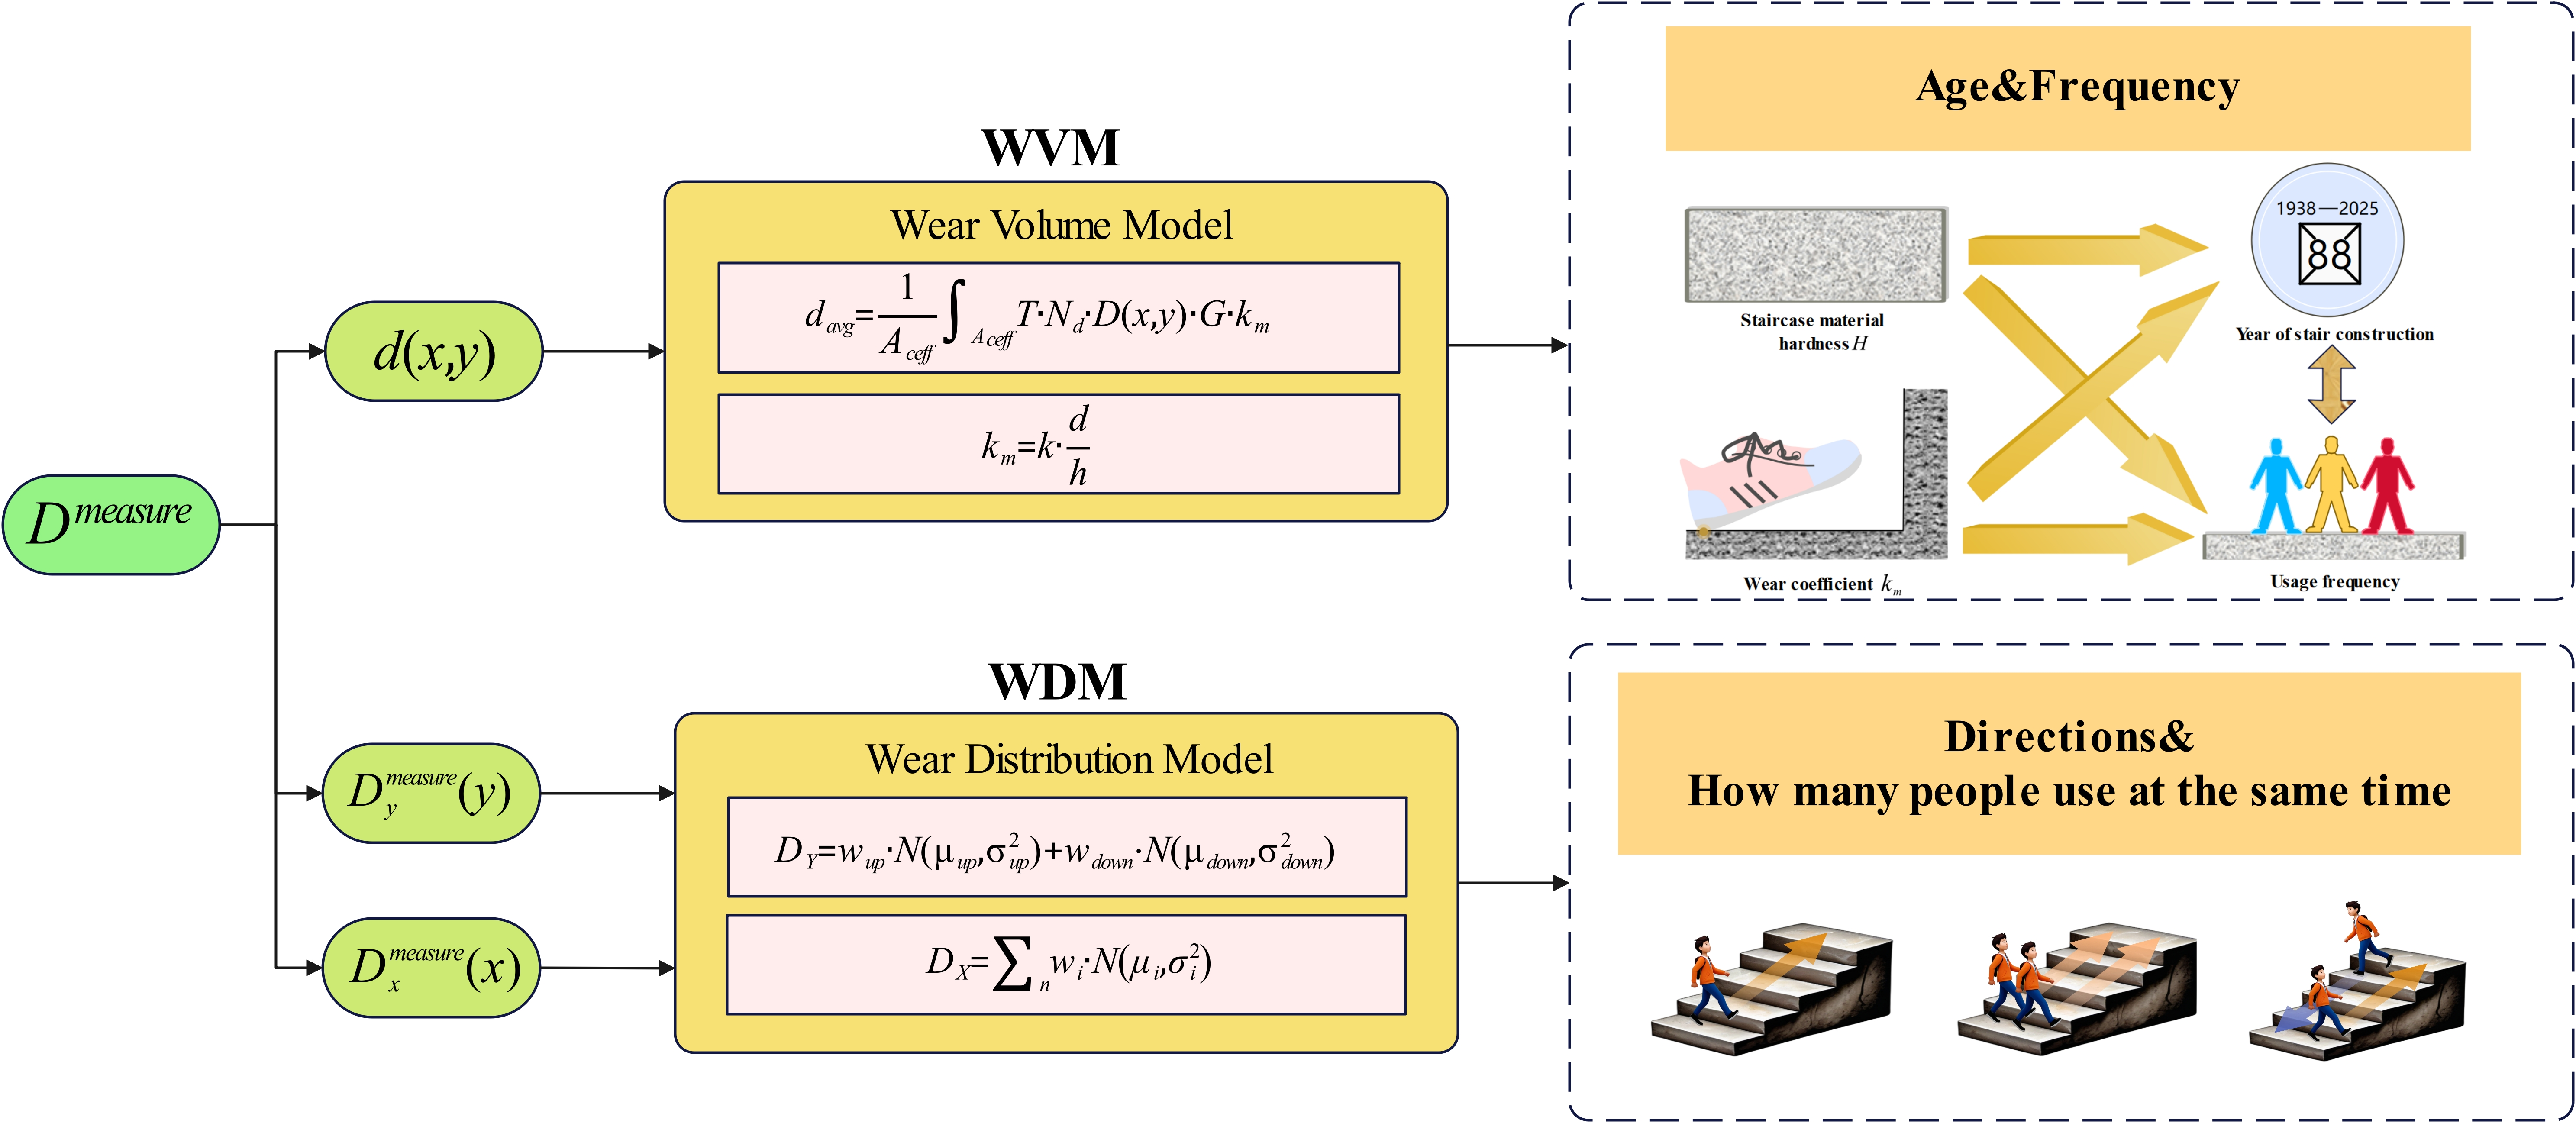
\includegraphics[width=\linewidth]{美赛Latex模板/模型流程图1.jpg}
	\caption{Flowchart for use by archaeological experts}
	\label{flowchart_Experts}
\end{figure}

\subsection{Solution of the Stair Wear Model}
In this section, we selected a set of ancient Edinburgh sand steps with a rectangular top-view surface. The rectangle is 2 meters long and 0.3 meter wide. Based on the 3D reconstruction of the image, we obtained the measurement matrix. Moreover, based on the information query, we obtained the rest of the required parameters as follows:

To solve the Wear Distribution Model, we design a Gauss Mixtual Algorithm. It can be used to respectively solve for normally distributed cumulants in the X and Y directions by wear measurement matrix $D^{measure}$. The exact flow of the algorithm is as follows:

\begin{table}[H]
    \centering
    \renewcommand{\arraystretch}{1.5}
    \setlength{\tabcolsep}{16pt}
    \begin{tabular}{>{\raggedright\arraybackslash}p{15cm}} 
        \hline
        \textbf{Gauss Mixtual Algorithm}\\ 
        \hline
        \textbf{Input:}\quad Wear measurement matrix $D^{measure}$\\  %Length $X$, Width $Y$?
        \textbf{Output:}\quad $P(D_X\mid\theta_k^{epoch})$ and $P(D_Y\mid\theta^{epoch})$ \\
        \(k = 0\) , \(\varepsilon = 1e-3\)\\
        while \(loss>\varepsilon\)\\ 
        \qquad for \(t\) in range($epoch$)\\ 
       \qquad\qquad \(\theta^{t+1}=
{\partial P(D_X\mid\theta^{t})}/{\partial \theta^t}
\), where $\theta=[ m_i,\mu_i,\sigma_i ]$\\
       \qquad\qquad $P(D_X\mid\theta^{t+1})=\sum_{i=1}^{k}m_i^{t+1}\cdot{N(\mu_i^{t+1},\sigma_i^{t+1})}$\\
      \qquad $loss = \Vert P(D_X\mid\theta_k^{epoch})-D_X \Vert$ \\

\(k = 2\)\\
for \(t\) in range($epoch$)\\ 
       \qquad \(\theta^{t+1}=
{\partial P(D_Y\mid\theta^{t})}/{\partial \theta^t}
\)\\
    \qquad $P(D_X\mid\theta^{t+1})=m_{up}^{t+1}\cdot{N(\mu_up^{t+1},\sigma_up^{t+1})}+m_{down}^{t+1}\cdot{N(\mu_down^{t+1},\sigma_down^{t+1})}$\\
       end\\
        \hline
    \end{tabular}
    \vspace{-0.8em}
\end{table}
Bringing $D^{measure}$ of the  Edinburgh sand step into the Gauss Mixtual Algorithm, we obtain the following normal distribution parameters. The parameters for the X and Y directions are placed in Table \ref{X_TABLE} and Table \ref{Y_TABLE} respectively.

\vspace{-2em}
\begin{minipage}[t]{0.5\linewidth}%第一栏尺寸
        \begin{table}[H]
    	    \centering
            \caption{\centering Normal distribution parameters in X direction}
            \vspace{-1em}
            \begin{figure}[H]
        	\centering
        	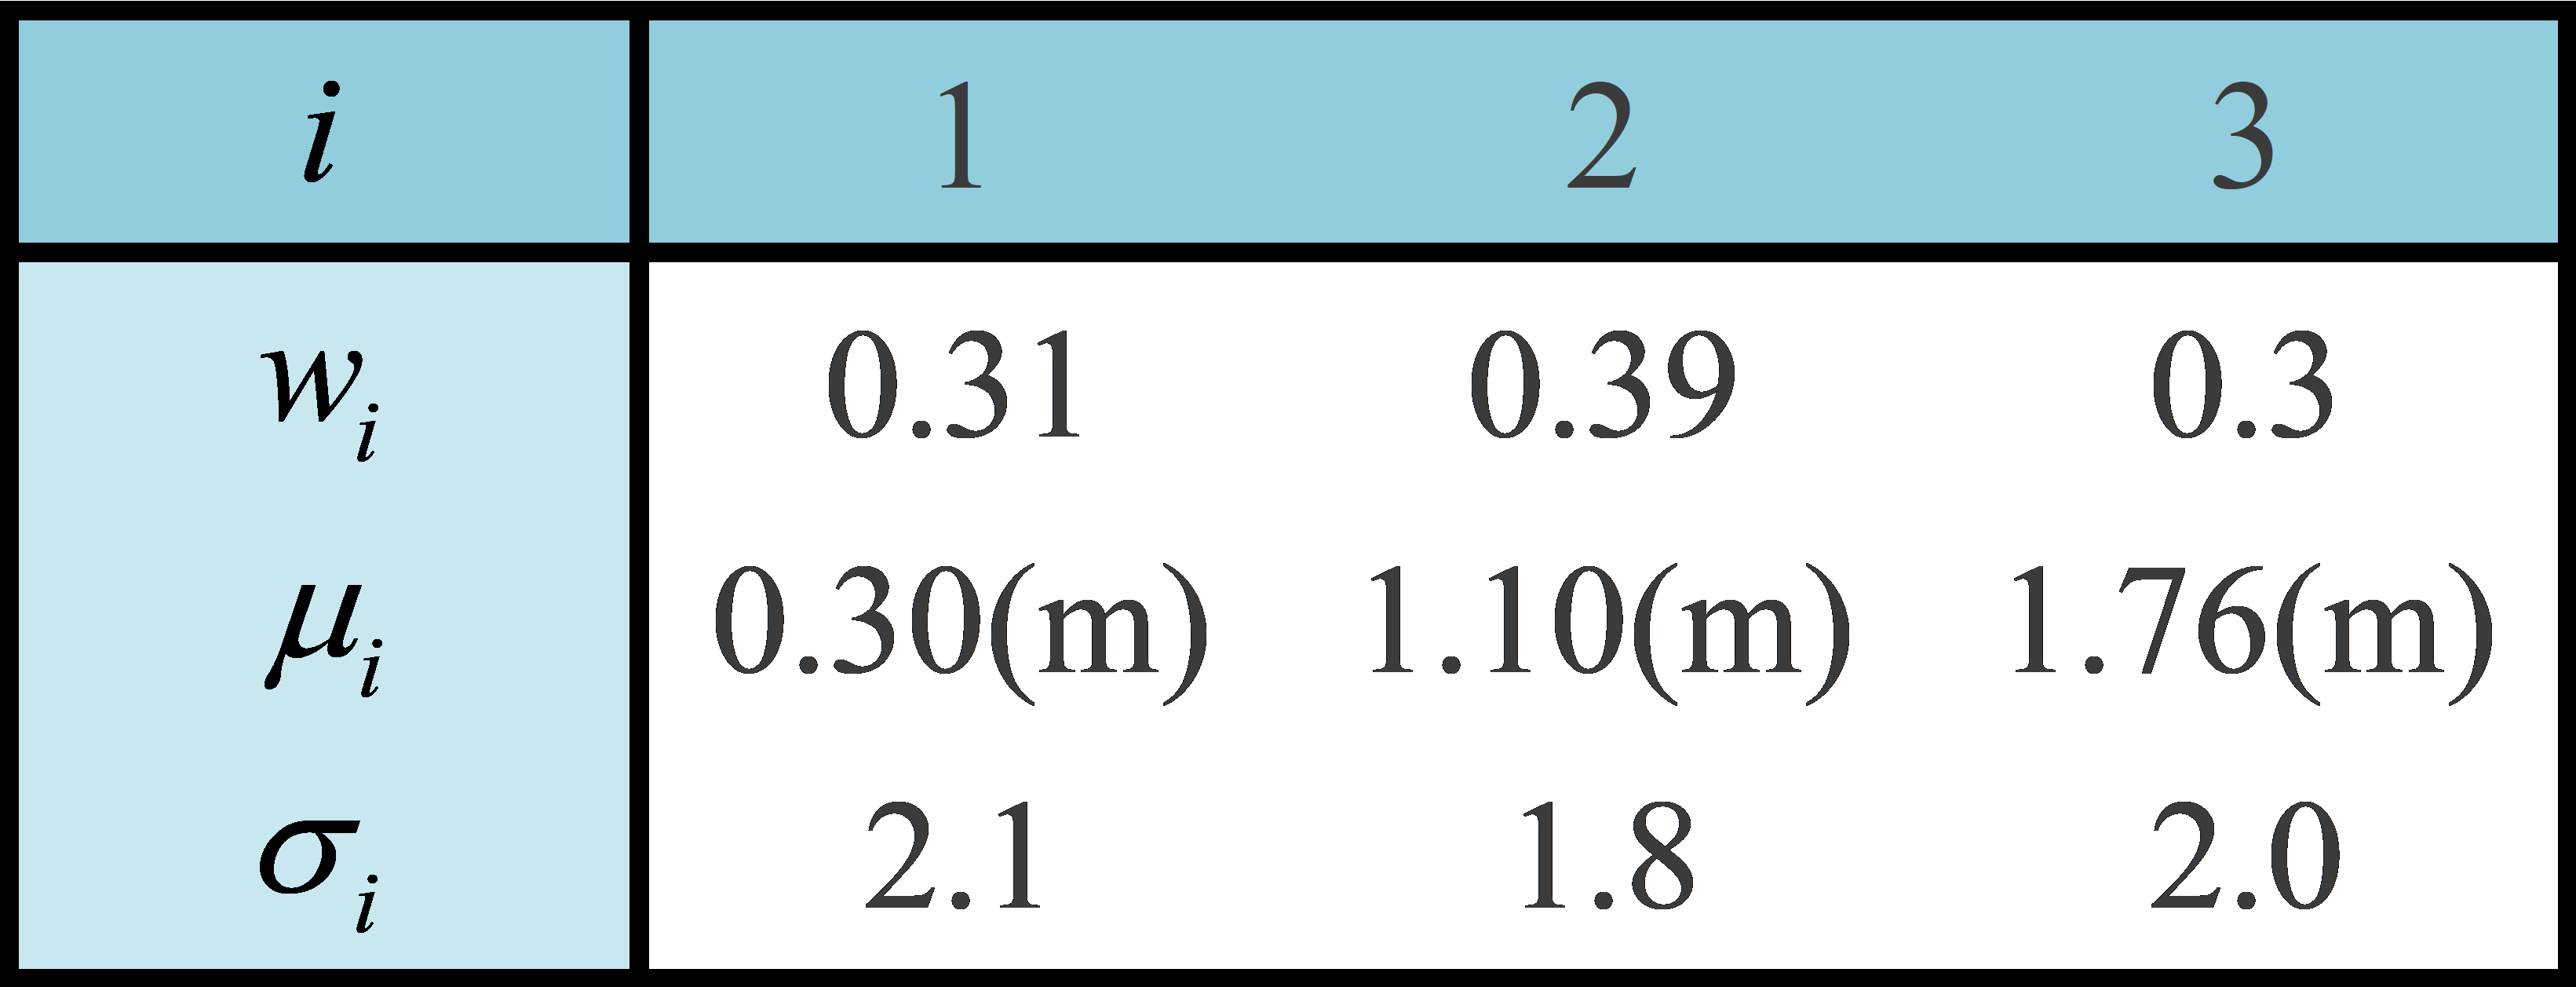
\includegraphics[width=1\textwidth]{X_TABLE.png}
        \end{figure}
        \label{X_TABLE}%设置专属标签,方便引用
        \end{table}
    \end{minipage}%第一栏结束
    \begin{minipage}[t]{0.5\linewidth}%第二栏尺寸
        \begin{table}[H]
    	    \centering
            \caption{\centering Normal distribution parameters in Y direction}
            \vspace{-1em}
            \begin{figure}[H]
        	\centering
        	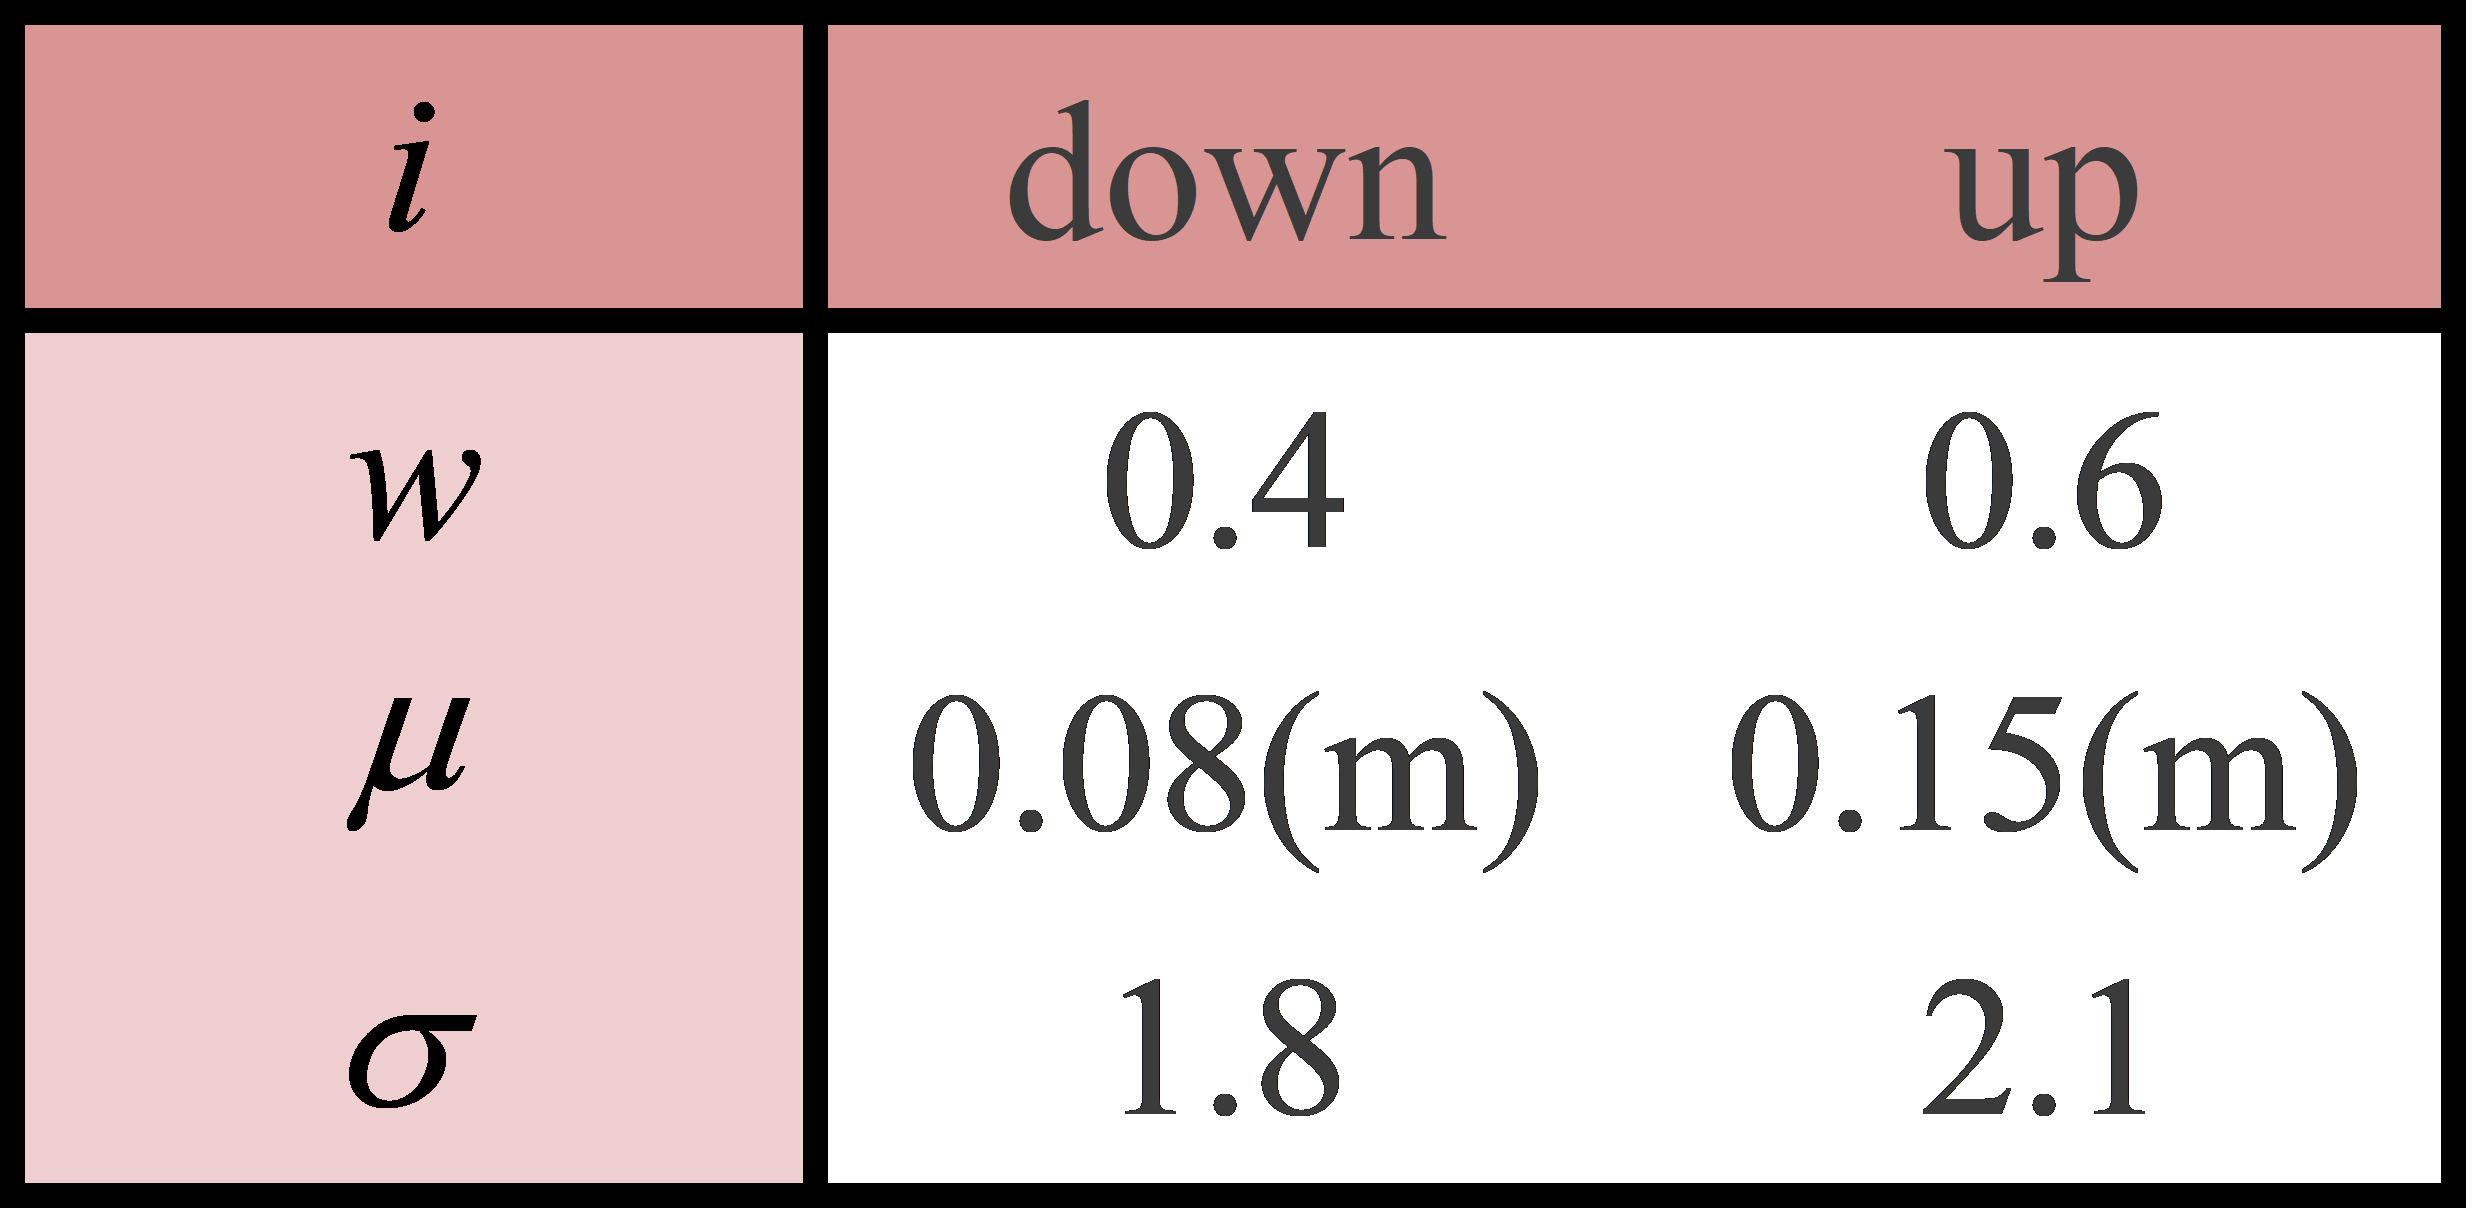
\includegraphics[width=0.77\textwidth]{Y_TABLE.png}
        \end{figure}
        \label{Y_TABLE}%设置专属标签,方便引用
        \end{table}
         \vspace{-2em}
    \end{minipage}\par %第二栏结束

From  Table \ref{X_TABLE} and Table \ref{Y_TABLE}, we can draw the conclusions that
\begin{enumerate}[\bfseries 1.]
	\setlength{\parsep}{0ex} %段落间距
	\setlength{\topsep}{-1ex} %列表到上下文的垂直距离
	\setlength{\itemsep}{0ex} %条目间距
	\item The wear distribution in the x-direction is accumulated from three normal distributions. The mean values of the three normal distributions are 0.30m, 1.10m and 1.76m. They are respectively on the left, centre and right side of the step. This reveals that \textbf{three people usually walked side by side on this step}. This may also show that the stair had a high flow of people.
	\item Of the three normal distributions in the x-direction, the second one has the highest probability and the smallest standard deviation. This indicates that people most often walked down the \textbf{middle} of the stairs. 
	\item Two normal distributions form a wear distribution in the Y-direction. \textbf{The stair was used in two direction}. The probability ratio of the number of people in the upward and downward direction was \textbf{3 : 2}. 
 %The standard deviation of the normal distribution corresponding to the upward direction is larger than that of the downward direction. 
 It means that the number of people in the \textbf{upward} row is \textbf{greater} than the number of people in the \textbf{downward} row.
     \item The mean of upward direction is 0.08m, while that of downward direction is 0.12m. They both close to the edge side of the step. Moreover, the mean of upward direction is closer to the edge of the step than the downward direction. This is consistent with our analysis.
\end{enumerate}
\vspace{-1em}

To describe the results of this set of steps more intuitively, we visualize the wear distribution of the steps and present them in \autoref{stepwear3}.
\begin{figure}[H]
\vspace{-1em}
	\centering
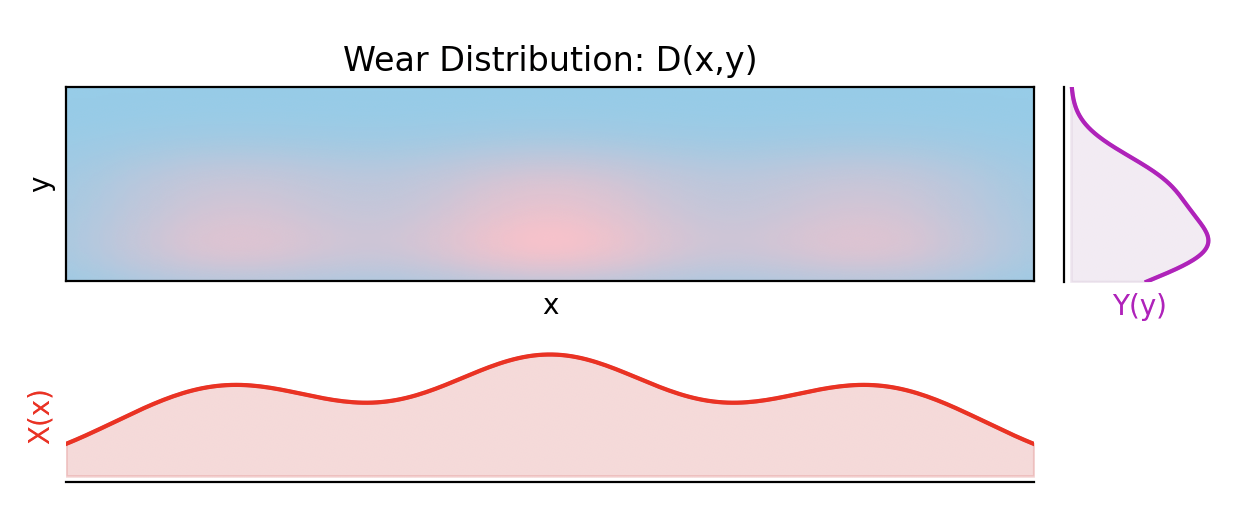
\includegraphics[width=0.8\linewidth]{美赛Latex模板/stepwear3.png}
	\caption{Visualization of step wear distribution}
	\label{stepwear3}
 \vspace{-1em}
\end{figure}
This graph gives the same conclusion. It visually presents that there are 3 peaks in the x-direction, indicating that there people usually walked side-by-side on it. There are two peaks in the y-direction. The peak corresponding to the downward direction is smaller than that of the upward direction. This suggests that the staircase was used in double direction.

After obtaining the wear distribution, combined with the parameters in Table (), the gradient age and frequency of use can be solved for each other. For this set of ancient Edinburgh sandstone steps, it is determined that this set of steps was constructed in a century ago. according to \autoref{MVM}, we can have that 
\begin{equation}
     N_d = \frac{A_{ceff}\cdot{d_{avg}}}{T\cdot{G}\cdot{k_m}}=261
\end{equation}
 This means that 261 people walked on it every day in the past. On the contary, when we consider that there were 260 people walked on it per day, the steps were constructed 36492 days ago.


\section{Solutions of Further Questions}

\subsection{Consistency of Wear Results}
\subsection{The Age of the Stairwell and Reliability}
\subsection{Repairs or renovations }
\subsection{the Source of the Material}
\subsection{People Use the Stair on A Typical Day}




\begin{equation}
    \delta{K}=\left | k_m-k_m^{t}\right|
\end{equation}

%时间推测
\begin{equation}
    T=\frac{d_{avg}}{N_d}\cdot{G}{k_m}
\end{equation}

%可靠性公式
\begin{equation}
    R=\frac{RA}{RA+RC}
\end{equation}

\section{Sensitivity Analysis}
\section{Strength and Weakness}
\section{Conclusion}

% 以下为信件/备忘录部分,不需要可自行去掉
% 如有需要可将整个 letter 环境移动到文章开头或中间
% 请在后一个花括号内填写信件(Letter)或备忘录(Memorandum)标题
%审视艺术家和流派的进化和革命趋势
%\begin{letter}{A document to the ICM Society}
%	\begin{flushleft}  % 左对齐环境,无首行缩进
%	To whom it may concern,
%	\end{flushleft}
%]
%\hfill Yours Sincerely,
%\hfill Team $\#$2107542  
%\end{letter}

\clearpage
\begin{thebibliography}{99}
	\bibitem{1} Yu, Xiao, Ruo-Xuan Ji, Yuan Chang, Chao Shen, Hui-Hong Guo, Xin-Li Xia, Wei-Lun Yin, and Chao Liu. "Growth Stability of Four Drought Resistant Plant Species in Different Regions." Ying Yong Sheng Tai Xue Bao 32.12 (2021): 4212-222. Web.
	\bibitem{2} Luo, Ruiping, and Benjamin Gilbert. "Timing of Short-term Drought Structures Plant-herbivore Dynamics." Oikos 2022.1 (2022): N/a. Web.
	\bibitem{3} Yang Haotian, Li Xinrong, Liu Lichao, Jia Rongliang, Wang Zengru, Li Xiaojun, Li Gang. Biomass allocation of four shrubs in desert grassland [J]. Journal of Desert Research,2013,33(5):1340-1348 (Chinese)
	\bibitem{4}  Farooq, M., A. Wahid, N. Kobayashi, D. Fujita, and S. M. A. Basra. "Plant Drought Stress: Effects, Mechanisms and Management." Agronomy for Sustainable Development 29.1 (2009): 185-212. Web.
	\bibitem{5}Patel, Jaykumar, and Avinash Mishra. "Plant Aquaporins Alleviate Drought Tolerance in Plants by Modulating Cellular Biochemistry, Root-architecture, and Photosynthesis." Physiologia Plantarum 172.2 (2021): 1030-044. Web.
	\bibitem{6}Descamps, Charlotte, Muriel Quinet, and Anne-Laure Jacquemart. "The Effects of Drought on Plant-pollinator Interactions: What to Expect?" Environmental and Experimental Botany 182(2021): 104297. Web.

\end{thebibliography}

\end{document}  % 结束$